\documentclass[twoside]{book}

% Packages required by doxygen
\usepackage{calc}
\usepackage{doxygen}
\usepackage{graphicx}
\usepackage[utf8]{inputenc}
\usepackage{makeidx}
\usepackage{multicol}
\usepackage{multirow}
\usepackage{textcomp}
\usepackage[table]{xcolor}

% NLS support packages
\usepackage[spanish]{babel}
% Font selection
\usepackage[T1]{fontenc}
\usepackage{mathptmx}
\usepackage[scaled=.90]{helvet}
\usepackage{courier}
\usepackage{amssymb}
\usepackage{sectsty}
\renewcommand{\familydefault}{\sfdefault}
\allsectionsfont{%
  \fontseries{bc}\selectfont%
  \color{darkgray}%
}
\renewcommand{\DoxyLabelFont}{%
  \fontseries{bc}\selectfont%
  \color{darkgray}%
}

% Page & text layout
\usepackage{geometry}
\geometry{%
  a4paper,%
  top=2.5cm,%
  bottom=2.5cm,%
  left=2.5cm,%
  right=2.5cm%
}
\tolerance=750
\hfuzz=15pt
\hbadness=750
\setlength{\emergencystretch}{15pt}
\setlength{\parindent}{0cm}
\setlength{\parskip}{0.2cm}
\makeatletter
\renewcommand{\paragraph}{%
  \@startsection{paragraph}{4}{0ex}{-1.0ex}{1.0ex}{%
    \normalfont\normalsize\bfseries\SS@parafont%
  }%
}
\renewcommand{\subparagraph}{%
  \@startsection{subparagraph}{5}{0ex}{-1.0ex}{1.0ex}{%
    \normalfont\normalsize\bfseries\SS@subparafont%
  }%
}
\makeatother

% Headers & footers
\usepackage{fancyhdr}
\pagestyle{fancyplain}
\fancyhead[LE]{\fancyplain{}{\bfseries\thepage}}
\fancyhead[CE]{\fancyplain{}{}}
\fancyhead[RE]{\fancyplain{}{\bfseries\leftmark}}
\fancyhead[LO]{\fancyplain{}{\bfseries\rightmark}}
\fancyhead[CO]{\fancyplain{}{}}
\fancyhead[RO]{\fancyplain{}{\bfseries\thepage}}
\fancyfoot[LE]{\fancyplain{}{}}
\fancyfoot[CE]{\fancyplain{}{}}
\fancyfoot[RE]{\fancyplain{}{\bfseries\scriptsize Generado el Domingo, 17 de Junio de 2018 19\-:48\-:21 para Memory+ por Doxygen }}
\fancyfoot[LO]{\fancyplain{}{\bfseries\scriptsize Generado el Domingo, 17 de Junio de 2018 19\-:48\-:21 para Memory+ por Doxygen }}
\fancyfoot[CO]{\fancyplain{}{}}
\fancyfoot[RO]{\fancyplain{}{}}
\renewcommand{\footrulewidth}{0.4pt}
\renewcommand{\chaptermark}[1]{%
  \markboth{#1}{}%
}
\renewcommand{\sectionmark}[1]{%
  \markright{\thesection\ #1}%
}

% Indices & bibliography
\usepackage{natbib}
\usepackage[titles]{tocloft}
\setcounter{tocdepth}{3}
\setcounter{secnumdepth}{5}
\makeindex

% Hyperlinks (required, but should be loaded last)
\usepackage{ifpdf}
\ifpdf
  \usepackage[pdftex,pagebackref=true]{hyperref}
\else
  \usepackage[ps2pdf,pagebackref=true]{hyperref}
\fi
\hypersetup{%
  colorlinks=true,%
  linkcolor=blue,%
  citecolor=blue,%
  unicode%
}

% Custom commands
\newcommand{\clearemptydoublepage}{%
  \newpage{\pagestyle{empty}\cleardoublepage}%
}


%===== C O N T E N T S =====

\begin{document}

% Titlepage & ToC
\hypersetup{pageanchor=false}
\pagenumbering{roman}
\begin{titlepage}
\vspace*{7cm}
\begin{center}%
{\Large Memory+ \\[1ex]\large 0.\-1 }\\
\vspace*{1cm}
{\large Generado por Doxygen 1.8.6}\\
\vspace*{0.5cm}
{\small Domingo, 17 de Junio de 2018 19:48:21}\\
\end{center}
\end{titlepage}
\clearemptydoublepage
\tableofcontents
\clearemptydoublepage
\pagenumbering{arabic}
\hypersetup{pageanchor=true}

%--- Begin generated contents ---
\chapter{Indice jerárquico}
\section{Jerarquía de la clase}
Esta lista de herencias esta ordenada aproximadamente por orden alfabético\-:\begin{DoxyCompactList}
\item Q\-Dialog\begin{DoxyCompactList}
\item \contentsline{section}{about}{\pageref{classabout}}{}
\item \contentsline{section}{game\-\_\-select}{\pageref{classgame__select}}{}
\end{DoxyCompactList}
\item Q\-Graphics\-Pixmap\-Item\begin{DoxyCompactList}
\item \contentsline{section}{Button}{\pageref{classButton}}{}
\item \contentsline{section}{Card}{\pageref{classCard}}{}
\end{DoxyCompactList}
\item Q\-Graphics\-View\begin{DoxyCompactList}
\item \contentsline{section}{Game\-\_\-c}{\pageref{classGame__c}}{}
\item \contentsline{section}{Game\-\_\-r}{\pageref{classGame__r}}{}
\end{DoxyCompactList}
\item Q\-Main\-Window\begin{DoxyCompactList}
\item \contentsline{section}{Main\-Window}{\pageref{classMainWindow}}{}
\end{DoxyCompactList}
\item Q\-Object\begin{DoxyCompactList}
\item \contentsline{section}{Button}{\pageref{classButton}}{}
\item \contentsline{section}{Card}{\pageref{classCard}}{}
\end{DoxyCompactList}
\end{DoxyCompactList}

\chapter{Índice de clases}
\section{Lista de clases}
Lista de las clases, estructuras, uniones e interfaces con una breve descripción\-:\begin{DoxyCompactList}
\item\contentsline{section}{\hyperlink{classabout}{about} }{\pageref{classabout}}{}
\item\contentsline{section}{\hyperlink{classButton}{Button} \\*Clase \hyperlink{classButton}{Button}. Hereda de Q\-Object y Q\-Graphics\-Pixmap\-Item }{\pageref{classButton}}{}
\item\contentsline{section}{\hyperlink{classCard}{Card} \\*Clase \hyperlink{classCard}{Card}. Hereda de Q\-Object y Q\-Graphics\-Pixmap\-Item }{\pageref{classCard}}{}
\item\contentsline{section}{\hyperlink{classGame__c}{Game\-\_\-c} \\*Clase \hyperlink{classGame__c}{Game\-\_\-c}. Hereda de Q\-Graphics\-View }{\pageref{classGame__c}}{}
\item\contentsline{section}{\hyperlink{classGame__r}{Game\-\_\-r} \\*Clase \hyperlink{classGame__r}{Game\-\_\-r}. Hereda de Q\-Graphics\-View }{\pageref{classGame__r}}{}
\item\contentsline{section}{\hyperlink{classgame__select}{game\-\_\-select} }{\pageref{classgame__select}}{}
\item\contentsline{section}{\hyperlink{classMainWindow}{Main\-Window} }{\pageref{classMainWindow}}{}
\end{DoxyCompactList}

\chapter{Indice de archivos}
\section{Lista de archivos}
Lista de todos los archivos documentados y con descripciones breves\-:\begin{DoxyCompactList}
\item\contentsline{section}{headers/\hyperlink{about_8h}{about.\-h} }{\pageref{about_8h}}{}
\item\contentsline{section}{headers/\hyperlink{aux__functions_8h}{aux\-\_\-functions.\-h} }{\pageref{aux__functions_8h}}{}
\item\contentsline{section}{headers/\hyperlink{button_8h}{button.\-h} }{\pageref{button_8h}}{}
\item\contentsline{section}{headers/\hyperlink{Card_8h}{Card.\-h} }{\pageref{Card_8h}}{}
\item\contentsline{section}{headers/\hyperlink{game__c_8h}{game\-\_\-c.\-h} }{\pageref{game__c_8h}}{}
\item\contentsline{section}{headers/\hyperlink{game__r_8h}{game\-\_\-r.\-h} }{\pageref{game__r_8h}}{}
\item\contentsline{section}{headers/\hyperlink{game__select_8h}{game\-\_\-select.\-h} }{\pageref{game__select_8h}}{}
\item\contentsline{section}{headers/\hyperlink{mainwindow_8h}{mainwindow.\-h} }{\pageref{mainwindow_8h}}{}
\item\contentsline{section}{source/\hyperlink{about_8cpp}{about.\-cpp} }{\pageref{about_8cpp}}{}
\item\contentsline{section}{source/\hyperlink{aux__functions_8cpp}{aux\-\_\-functions.\-cpp} }{\pageref{aux__functions_8cpp}}{}
\item\contentsline{section}{source/\hyperlink{button_8cpp}{button.\-cpp} }{\pageref{button_8cpp}}{}
\item\contentsline{section}{source/\hyperlink{game__c_8cpp}{game\-\_\-c.\-cpp} }{\pageref{game__c_8cpp}}{}
\item\contentsline{section}{source/\hyperlink{game__r_8cpp}{game\-\_\-r.\-cpp} }{\pageref{game__r_8cpp}}{}
\item\contentsline{section}{source/\hyperlink{game__select_8cpp}{game\-\_\-select.\-cpp} }{\pageref{game__select_8cpp}}{}
\item\contentsline{section}{source/\hyperlink{main_8cpp}{main.\-cpp} }{\pageref{main_8cpp}}{}
\item\contentsline{section}{source/\hyperlink{mainwindow_8cpp}{mainwindow.\-cpp} }{\pageref{mainwindow_8cpp}}{}
\end{DoxyCompactList}

\chapter{Documentación de las clases}
\hypertarget{classabout}{\section{Referencia de la Clase about}
\label{classabout}\index{about@{about}}
}
Diagrama de herencias de about\begin{figure}[H]
\begin{center}
\leavevmode
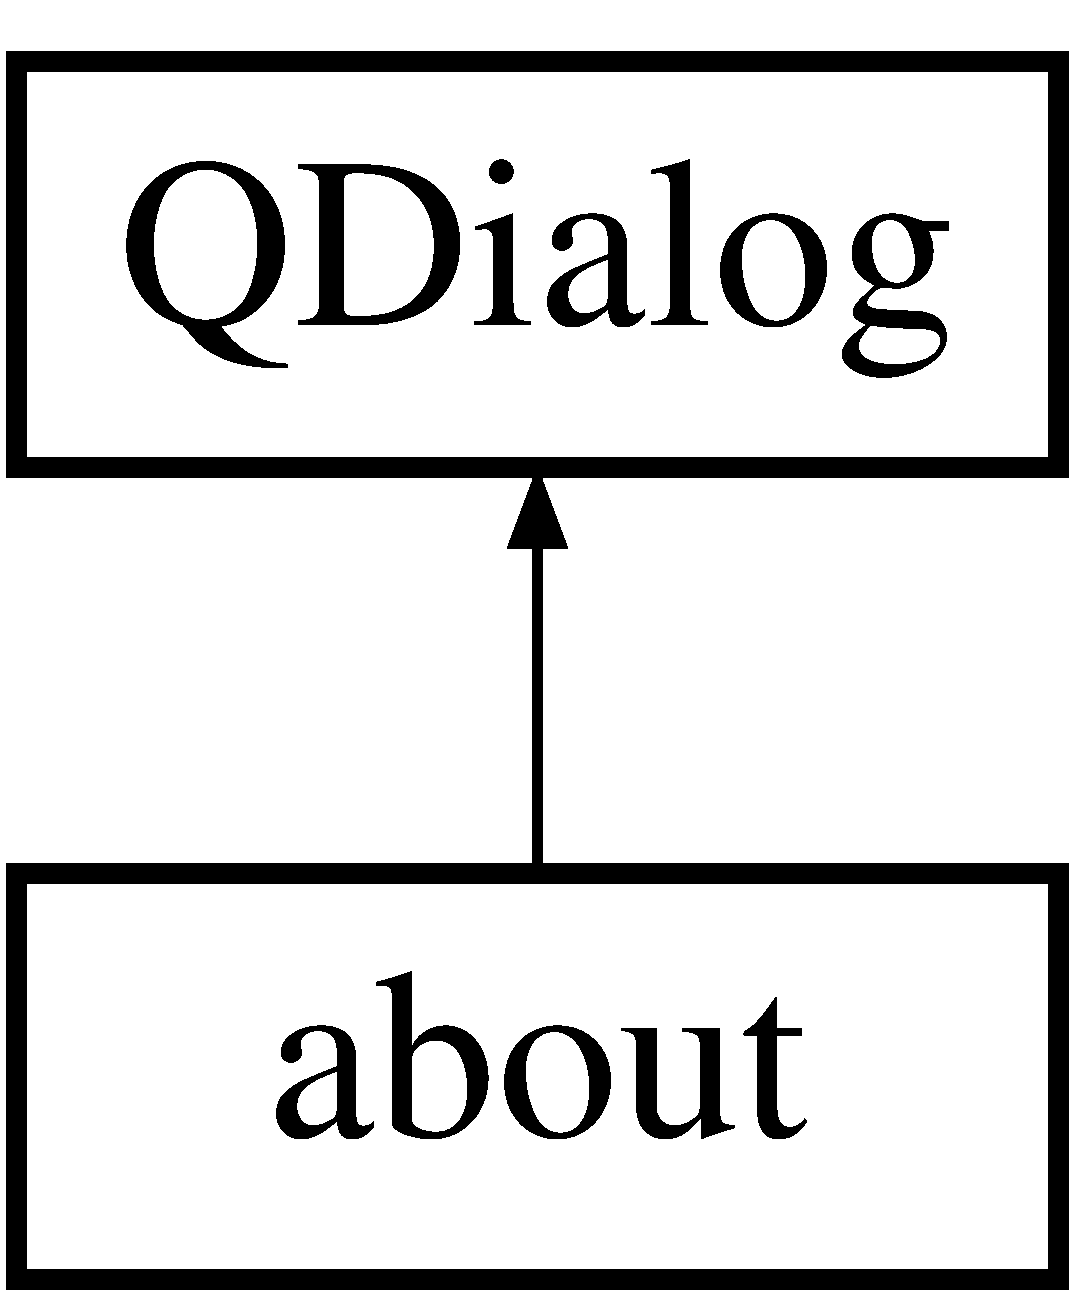
\includegraphics[height=2.000000cm]{classabout}
\end{center}
\end{figure}
\subsection*{Métodos públicos}
\begin{DoxyCompactItemize}
\item 
\hypertarget{classabout_ab16a8ec628d97aee17f0332e09964f52}{{\bfseries about} (Q\-Widget $\ast$parent=0)}\label{classabout_ab16a8ec628d97aee17f0332e09964f52}

\end{DoxyCompactItemize}


\subsection{Descripción detallada}


Definición en la línea 15 del archivo about.\-h.



La documentación para esta clase fue generada a partir de los siguientes ficheros\-:\begin{DoxyCompactItemize}
\item 
headers/\hyperlink{about_8h}{about.\-h}\item 
source/\hyperlink{about_8cpp}{about.\-cpp}\end{DoxyCompactItemize}

\hypertarget{classButton}{\section{Referencia de la Clase Button}
\label{classButton}\index{Button@{Button}}
}


Clase \hyperlink{classButton}{Button}. Hereda de Q\-Object y Q\-Graphics\-Pixmap\-Item.  




{\ttfamily \#include $<$button.\-h$>$}

Diagrama de herencias de Button\begin{figure}[H]
\begin{center}
\leavevmode
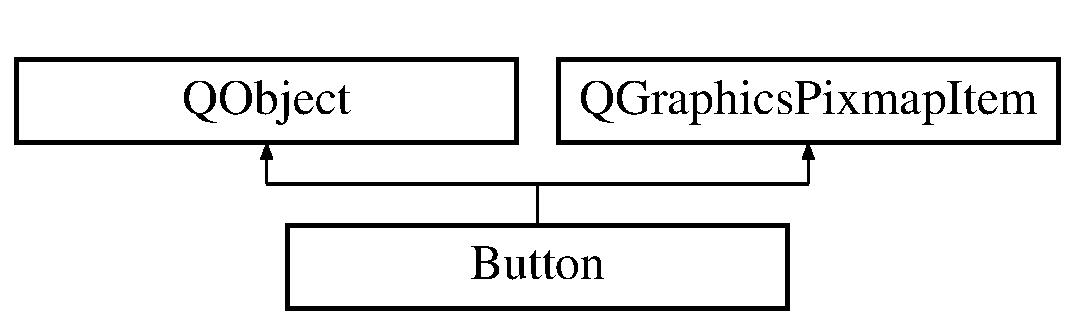
\includegraphics[height=2.000000cm]{classButton}
\end{center}
\end{figure}
\subsection*{Señales}
\begin{DoxyCompactItemize}
\item 
\hypertarget{classButton_a9e7ab4152cb1e7e3beb7f2842f32670c}{void {\bfseries clicked} ()}\label{classButton_a9e7ab4152cb1e7e3beb7f2842f32670c}

\end{DoxyCompactItemize}
\subsection*{Métodos públicos}
\begin{DoxyCompactItemize}
\item 
\hyperlink{classButton_aaa64acc02b613f8e480edb5040eb99d2}{Button} (Q\-String img\-\_\-standby, Q\-String img\-\_\-active, Q\-Graphics\-Item $\ast$parent=N\-U\-L\-L)
\begin{DoxyCompactList}\small\item\em Constructor de la clase \hyperlink{classButton}{Button}. \end{DoxyCompactList}\item 
void \hyperlink{classButton_a17d8eb0c904605b223bbc00c75655315}{mouse\-Press\-Event} (Q\-Graphics\-Scene\-Mouse\-Event $\ast$event)
\begin{DoxyCompactList}\small\item\em Emite la señal clicked() siempre que se pulsa el botón izquierdo del ratón sobre una instancia de la clase \hyperlink{classButton}{Button}. \end{DoxyCompactList}\item 
void \hyperlink{classButton_a633a9684818bc5d300a622a00064f09c}{hover\-Enter\-Event} (Q\-Graphics\-Scene\-Hover\-Event $\ast$event)
\begin{DoxyCompactList}\small\item\em Cambia la imagen del botón a su forma activa siempre que el cursor pasa por encima de una instancia de la clase \hyperlink{classButton}{Button}. \end{DoxyCompactList}\item 
void \hyperlink{classButton_a1689a97690d9469ce8350d24db0d7485}{hover\-Leave\-Event} (Q\-Graphics\-Scene\-Hover\-Event $\ast$event)
\begin{DoxyCompactList}\small\item\em Cambia la imagen del botón a su forma inactiva siempre que el cursor pasa por encima de una instancia de la clase \hyperlink{classButton}{Button}. \end{DoxyCompactList}\item 
void \hyperlink{classButton_a4706976fe64d05194702baa179fa99da}{set\-Images} (Q\-String img\-\_\-standby, Q\-String img\-\_\-active)
\begin{DoxyCompactList}\small\item\em Carga las imágenes del botón. \end{DoxyCompactList}\end{DoxyCompactItemize}


\subsection{Descripción detallada}
Clase \hyperlink{classButton}{Button}. Hereda de Q\-Object y Q\-Graphics\-Pixmap\-Item. 

Definición en la línea 18 del archivo button.\-h.



\subsection{Documentación del constructor y destructor}
\hypertarget{classButton_aaa64acc02b613f8e480edb5040eb99d2}{\index{Button@{Button}!Button@{Button}}
\index{Button@{Button}!Button@{Button}}
\subsubsection[{Button}]{\setlength{\rightskip}{0pt plus 5cm}Button\-::\-Button (
\begin{DoxyParamCaption}
\item[{Q\-String}]{img\-\_\-standby, }
\item[{Q\-String}]{img\-\_\-active, }
\item[{Q\-Graphics\-Item $\ast$}]{parent = {\ttfamily NULL}}
\end{DoxyParamCaption}
)}}\label{classButton_aaa64acc02b613f8e480edb5040eb99d2}


Constructor de la clase \hyperlink{classButton}{Button}. 


\begin{DoxyParams}{Parámetros}
{\em img\-\_\-standby} & Path de la imagen del botón en reposo. \\
\hline
{\em img\-\_\-active} & Path de la imagen del botón activo (hover). \\
\hline
{\em parent} & Puntero a Q\-Graphics\-Item a partir del cual fue creado el botón (por defecto es N\-U\-L\-L). \\
\hline
\end{DoxyParams}


Definición en la línea 9 del archivo button.\-cpp.



\subsection{Documentación de las funciones miembro}
\hypertarget{classButton_a633a9684818bc5d300a622a00064f09c}{\index{Button@{Button}!hover\-Enter\-Event@{hover\-Enter\-Event}}
\index{hover\-Enter\-Event@{hover\-Enter\-Event}!Button@{Button}}
\subsubsection[{hover\-Enter\-Event}]{\setlength{\rightskip}{0pt plus 5cm}void Button\-::hover\-Enter\-Event (
\begin{DoxyParamCaption}
\item[{Q\-Graphics\-Scene\-Hover\-Event $\ast$}]{event}
\end{DoxyParamCaption}
)}}\label{classButton_a633a9684818bc5d300a622a00064f09c}


Cambia la imagen del botón a su forma activa siempre que el cursor pasa por encima de una instancia de la clase \hyperlink{classButton}{Button}. 


\begin{DoxyParams}{Parámetros}
{\em event} & Puntero al evento generado por pasar el cursor del ratón sobre una instancia de this. \\
\hline
\end{DoxyParams}


Definición en la línea 23 del archivo button.\-cpp.

\hypertarget{classButton_a1689a97690d9469ce8350d24db0d7485}{\index{Button@{Button}!hover\-Leave\-Event@{hover\-Leave\-Event}}
\index{hover\-Leave\-Event@{hover\-Leave\-Event}!Button@{Button}}
\subsubsection[{hover\-Leave\-Event}]{\setlength{\rightskip}{0pt plus 5cm}void Button\-::hover\-Leave\-Event (
\begin{DoxyParamCaption}
\item[{Q\-Graphics\-Scene\-Hover\-Event $\ast$}]{event}
\end{DoxyParamCaption}
)}}\label{classButton_a1689a97690d9469ce8350d24db0d7485}


Cambia la imagen del botón a su forma inactiva siempre que el cursor pasa por encima de una instancia de la clase \hyperlink{classButton}{Button}. 


\begin{DoxyParams}{Parámetros}
{\em event} & Puntero al evento generado por pasar el cursor del ratón sobre una instancia de this. \\
\hline
\end{DoxyParams}


Definición en la línea 28 del archivo button.\-cpp.

\hypertarget{classButton_a17d8eb0c904605b223bbc00c75655315}{\index{Button@{Button}!mouse\-Press\-Event@{mouse\-Press\-Event}}
\index{mouse\-Press\-Event@{mouse\-Press\-Event}!Button@{Button}}
\subsubsection[{mouse\-Press\-Event}]{\setlength{\rightskip}{0pt plus 5cm}void Button\-::mouse\-Press\-Event (
\begin{DoxyParamCaption}
\item[{Q\-Graphics\-Scene\-Mouse\-Event $\ast$}]{event}
\end{DoxyParamCaption}
)}}\label{classButton_a17d8eb0c904605b223bbc00c75655315}


Emite la señal clicked() siempre que se pulsa el botón izquierdo del ratón sobre una instancia de la clase \hyperlink{classButton}{Button}. 


\begin{DoxyParams}{Parámetros}
{\em event} & Puntero al evento generado por pulsar un botón del ratón. \\
\hline
\end{DoxyParams}


Definición en la línea 17 del archivo button.\-cpp.

\hypertarget{classButton_a4706976fe64d05194702baa179fa99da}{\index{Button@{Button}!set\-Images@{set\-Images}}
\index{set\-Images@{set\-Images}!Button@{Button}}
\subsubsection[{set\-Images}]{\setlength{\rightskip}{0pt plus 5cm}void Button\-::set\-Images (
\begin{DoxyParamCaption}
\item[{Q\-String}]{img\-\_\-standby, }
\item[{Q\-String}]{img\-\_\-active}
\end{DoxyParamCaption}
)}}\label{classButton_a4706976fe64d05194702baa179fa99da}


Carga las imágenes del botón. 


\begin{DoxyParams}{Parámetros}
{\em img\-\_\-standby} & Path de la imagen del botón en reposo. \\
\hline
{\em img\-\_\-active} & Path de la imagen del botón activo (hover). \\
\hline
\end{DoxyParams}


Definición en la línea 33 del archivo button.\-cpp.



La documentación para esta clase fue generada a partir de los siguientes ficheros\-:\begin{DoxyCompactItemize}
\item 
headers/\hyperlink{button_8h}{button.\-h}\item 
source/\hyperlink{button_8cpp}{button.\-cpp}\end{DoxyCompactItemize}

\hypertarget{classCard}{\section{Referencia de la Clase Card}
\label{classCard}\index{Card@{Card}}
}


Clase \hyperlink{classCard}{Card}. Hereda de Q\-Object y Q\-Graphics\-Pixmap\-Item.  




{\ttfamily \#include $<$Card.\-h$>$}

Diagrama de herencias de Card\begin{figure}[H]
\begin{center}
\leavevmode
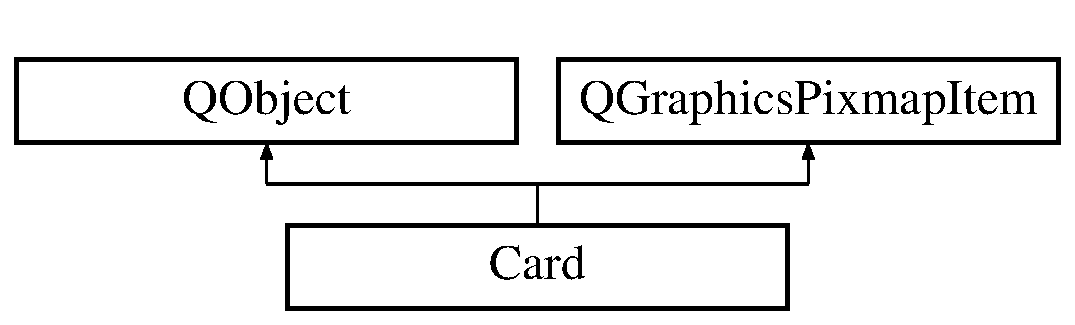
\includegraphics[height=2.000000cm]{classCard}
\end{center}
\end{figure}
\subsection*{Métodos públicos}
\begin{DoxyCompactItemize}
\item 
\hyperlink{classCard_a7340a365f3fbe880a434c68d7e665a33}{Card} (Q\-String dorsal, Q\-String up, int id=-\/1, Q\-Graphics\-Item $\ast$parent=N\-U\-L\-L)
\begin{DoxyCompactList}\small\item\em Constructor de la clase. \end{DoxyCompactList}\item 
void \hyperlink{classCard_a5ccb7a98359b49bdaac475e8b2129975}{set\-\_\-card} (Q\-String dorsal, Q\-String up, int id)
\begin{DoxyCompactList}\small\item\em Modifica las imágenes de la carta. \end{DoxyCompactList}\item 
\hypertarget{classCard_abbd46606b409c7981a9defb38c8a29b8}{void \hyperlink{classCard_abbd46606b409c7981a9defb38c8a29b8}{show\-\_\-card} ()}\label{classCard_abbd46606b409c7981a9defb38c8a29b8}

\begin{DoxyCompactList}\small\item\em Coloca al frente la imagen frontal de la carta. \end{DoxyCompactList}\item 
\hypertarget{classCard_ac9821ebe4235b9dac41055e58675a4a5}{void \hyperlink{classCard_ac9821ebe4235b9dac41055e58675a4a5}{hide\-\_\-card} ()}\label{classCard_ac9821ebe4235b9dac41055e58675a4a5}

\begin{DoxyCompactList}\small\item\em Coloca al frente la imagen dorsal de la carta. \end{DoxyCompactList}\item 
Q\-Pixmap \hyperlink{classCard_a7f255cbb86ac67fde3dfcbd27e1b2b30}{get\-\_\-dorsal} ()
\begin{DoxyCompactList}\small\item\em Retorna la imagen dorsal de la carta. \end{DoxyCompactList}\item 
Q\-Pixmap \hyperlink{classCard_adbf014c1fb61e64aeea10d5ca448a10d}{get\-\_\-front} ()
\begin{DoxyCompactList}\small\item\em Retorna la imagen frontal de la carta. \end{DoxyCompactList}\item 
int \hyperlink{classCard_a56b662276984f1e4493cd3bd708915a9}{get\-\_\-id} ()
\begin{DoxyCompactList}\small\item\em Retorna el id de la carta. \end{DoxyCompactList}\item 
Q\-String \hyperlink{classCard_a5e15f19d3da91a951e38319ae0a30999}{get\-\_\-name} (size\-\_\-t index)
\begin{DoxyCompactList}\small\item\em Retorna el path de la imagen de la carta según un índice (0 o 1). \end{DoxyCompactList}\item 
void \hyperlink{classCard_a57dcb9478cf6fe08b492cb035a33fd5d}{set\-\_\-id} (int id)
\begin{DoxyCompactList}\small\item\em Modifica el id de la carta. \end{DoxyCompactList}\item 
bool \hyperlink{classCard_a9ebc44fd37f1a6633d3b5c26d74aa185}{is\-\_\-up} ()
\begin{DoxyCompactList}\small\item\em Comprueba si la carta está hacia arriba (frontal) o hacia abajo (dorsal). \end{DoxyCompactList}\end{DoxyCompactItemize}
\subsection*{Métodos protegidos}
\begin{DoxyCompactItemize}
\item 
void \hyperlink{classCard_a731947ca9a438d2af418586414b3e2c9}{mouse\-Press\-Event} (Q\-Graphics\-Scene\-Mouse\-Event $\ast$event)
\begin{DoxyCompactList}\small\item\em Muestra u oculta la carta cuando recibe un click con el botón izquierdo del ratón. \end{DoxyCompactList}\end{DoxyCompactItemize}


\subsection{Descripción detallada}
Clase \hyperlink{classCard}{Card}. Hereda de Q\-Object y Q\-Graphics\-Pixmap\-Item. 

Definición en la línea 17 del archivo Card.\-h.



\subsection{Documentación del constructor y destructor}
\hypertarget{classCard_a7340a365f3fbe880a434c68d7e665a33}{\index{Card@{Card}!Card@{Card}}
\index{Card@{Card}!Card@{Card}}
\subsubsection[{Card}]{\setlength{\rightskip}{0pt plus 5cm}Card\-::\-Card (
\begin{DoxyParamCaption}
\item[{Q\-String}]{dorsal, }
\item[{Q\-String}]{up, }
\item[{int}]{id = {\ttfamily -\/1}, }
\item[{Q\-Graphics\-Item $\ast$}]{parent = {\ttfamily NULL}}
\end{DoxyParamCaption}
)\hspace{0.3cm}{\ttfamily [inline]}}}\label{classCard_a7340a365f3fbe880a434c68d7e665a33}


Constructor de la clase. 


\begin{DoxyParams}{Parámetros}
{\em dorsal} & Cadena de texto con el path de la imagen dorsal de la carta. \\
\hline
{\em up} & Cadena de texto con el path de la imagen frontal de la carta. \\
\hline
{\em id} & Número que identifica la carta. \\
\hline
{\em parent} & \\
\hline
\end{DoxyParams}


Definición en la línea 36 del archivo Card.\-h.



\subsection{Documentación de las funciones miembro}
\hypertarget{classCard_a7f255cbb86ac67fde3dfcbd27e1b2b30}{\index{Card@{Card}!get\-\_\-dorsal@{get\-\_\-dorsal}}
\index{get\-\_\-dorsal@{get\-\_\-dorsal}!Card@{Card}}
\subsubsection[{get\-\_\-dorsal}]{\setlength{\rightskip}{0pt plus 5cm}Q\-Pixmap Card\-::get\-\_\-dorsal (
\begin{DoxyParamCaption}
{}
\end{DoxyParamCaption}
)\hspace{0.3cm}{\ttfamily [inline]}}}\label{classCard_a7f255cbb86ac67fde3dfcbd27e1b2b30}


Retorna la imagen dorsal de la carta. 

\begin{DoxyReturn}{Devuelve}
Imagen dorsal de la carta. 
\end{DoxyReturn}


Definición en la línea 84 del archivo Card.\-h.

\hypertarget{classCard_adbf014c1fb61e64aeea10d5ca448a10d}{\index{Card@{Card}!get\-\_\-front@{get\-\_\-front}}
\index{get\-\_\-front@{get\-\_\-front}!Card@{Card}}
\subsubsection[{get\-\_\-front}]{\setlength{\rightskip}{0pt plus 5cm}Q\-Pixmap Card\-::get\-\_\-front (
\begin{DoxyParamCaption}
{}
\end{DoxyParamCaption}
)\hspace{0.3cm}{\ttfamily [inline]}}}\label{classCard_adbf014c1fb61e64aeea10d5ca448a10d}


Retorna la imagen frontal de la carta. 

\begin{DoxyReturn}{Devuelve}
Imagen frontal de la carta. 
\end{DoxyReturn}


Definición en la línea 93 del archivo Card.\-h.

\hypertarget{classCard_a56b662276984f1e4493cd3bd708915a9}{\index{Card@{Card}!get\-\_\-id@{get\-\_\-id}}
\index{get\-\_\-id@{get\-\_\-id}!Card@{Card}}
\subsubsection[{get\-\_\-id}]{\setlength{\rightskip}{0pt plus 5cm}int Card\-::get\-\_\-id (
\begin{DoxyParamCaption}
{}
\end{DoxyParamCaption}
)\hspace{0.3cm}{\ttfamily [inline]}}}\label{classCard_a56b662276984f1e4493cd3bd708915a9}


Retorna el id de la carta. 

\begin{DoxyReturn}{Devuelve}
id de la carta. 
\end{DoxyReturn}


Definición en la línea 102 del archivo Card.\-h.

\hypertarget{classCard_a5e15f19d3da91a951e38319ae0a30999}{\index{Card@{Card}!get\-\_\-name@{get\-\_\-name}}
\index{get\-\_\-name@{get\-\_\-name}!Card@{Card}}
\subsubsection[{get\-\_\-name}]{\setlength{\rightskip}{0pt plus 5cm}Q\-String Card\-::get\-\_\-name (
\begin{DoxyParamCaption}
\item[{size\-\_\-t}]{index}
\end{DoxyParamCaption}
)\hspace{0.3cm}{\ttfamily [inline]}}}\label{classCard_a5e15f19d3da91a951e38319ae0a30999}


Retorna el path de la imagen de la carta según un índice (0 o 1). 


\begin{DoxyParams}{Parámetros}
{\em index} & Índice del arreglo que contiene los path's de las imágenes. \\
\hline
\end{DoxyParams}
\begin{DoxyReturn}{Devuelve}
Path de la imagen si el índice es 0 o 1. 

Cadena vacia si el índice es diferente de 0 y 1. 
\end{DoxyReturn}


Definición en la línea 113 del archivo Card.\-h.

\hypertarget{classCard_a9ebc44fd37f1a6633d3b5c26d74aa185}{\index{Card@{Card}!is\-\_\-up@{is\-\_\-up}}
\index{is\-\_\-up@{is\-\_\-up}!Card@{Card}}
\subsubsection[{is\-\_\-up}]{\setlength{\rightskip}{0pt plus 5cm}bool Card\-::is\-\_\-up (
\begin{DoxyParamCaption}
{}
\end{DoxyParamCaption}
)\hspace{0.3cm}{\ttfamily [inline]}}}\label{classCard_a9ebc44fd37f1a6633d3b5c26d74aa185}


Comprueba si la carta está hacia arriba (frontal) o hacia abajo (dorsal). 

\begin{DoxyReturn}{Devuelve}
true si la carta está hacia arriba. 

false si la carta está hacia abajo. 
\end{DoxyReturn}


Definición en la línea 135 del archivo Card.\-h.

\hypertarget{classCard_a731947ca9a438d2af418586414b3e2c9}{\index{Card@{Card}!mouse\-Press\-Event@{mouse\-Press\-Event}}
\index{mouse\-Press\-Event@{mouse\-Press\-Event}!Card@{Card}}
\subsubsection[{mouse\-Press\-Event}]{\setlength{\rightskip}{0pt plus 5cm}void Card\-::mouse\-Press\-Event (
\begin{DoxyParamCaption}
\item[{Q\-Graphics\-Scene\-Mouse\-Event $\ast$}]{event}
\end{DoxyParamCaption}
)\hspace{0.3cm}{\ttfamily [inline]}, {\ttfamily [protected]}}}\label{classCard_a731947ca9a438d2af418586414b3e2c9}


Muestra u oculta la carta cuando recibe un click con el botón izquierdo del ratón. 


\begin{DoxyParams}{Parámetros}
{\em event} & Evento que se genera al hacer click con el ratón sobre la carta. \\
\hline
\end{DoxyParams}


Definición en la línea 149 del archivo Card.\-h.

\hypertarget{classCard_a5ccb7a98359b49bdaac475e8b2129975}{\index{Card@{Card}!set\-\_\-card@{set\-\_\-card}}
\index{set\-\_\-card@{set\-\_\-card}!Card@{Card}}
\subsubsection[{set\-\_\-card}]{\setlength{\rightskip}{0pt plus 5cm}void Card\-::set\-\_\-card (
\begin{DoxyParamCaption}
\item[{Q\-String}]{dorsal, }
\item[{Q\-String}]{up, }
\item[{int}]{id}
\end{DoxyParamCaption}
)\hspace{0.3cm}{\ttfamily [inline]}}}\label{classCard_a5ccb7a98359b49bdaac475e8b2129975}


Modifica las imágenes de la carta. 


\begin{DoxyParams}{Parámetros}
{\em dorsal} & Cadena de texto con el path de la imagen dorsal de la carta. \\
\hline
{\em up} & Cadena de texto con el path de la imagen frontal de la carta. \\
\hline
{\em id} & Número que identifica la carta. \\
\hline
\end{DoxyParams}


Definición en la línea 53 del archivo Card.\-h.

\hypertarget{classCard_a57dcb9478cf6fe08b492cb035a33fd5d}{\index{Card@{Card}!set\-\_\-id@{set\-\_\-id}}
\index{set\-\_\-id@{set\-\_\-id}!Card@{Card}}
\subsubsection[{set\-\_\-id}]{\setlength{\rightskip}{0pt plus 5cm}void Card\-::set\-\_\-id (
\begin{DoxyParamCaption}
\item[{int}]{id}
\end{DoxyParamCaption}
)\hspace{0.3cm}{\ttfamily [inline]}}}\label{classCard_a57dcb9478cf6fe08b492cb035a33fd5d}


Modifica el id de la carta. 


\begin{DoxyParams}{Parámetros}
{\em id} & Número que identifica a la carta. \\
\hline
\end{DoxyParams}


Definición en la línea 125 del archivo Card.\-h.



La documentación para esta clase fue generada a partir del siguiente fichero\-:\begin{DoxyCompactItemize}
\item 
headers/\hyperlink{Card_8h}{Card.\-h}\end{DoxyCompactItemize}

\hypertarget{classGame__c}{\section{Referencia de la Clase Game\-\_\-c}
\label{classGame__c}\index{Game\-\_\-c@{Game\-\_\-c}}
}


Clase \hyperlink{classGame__c}{Game\-\_\-c}. Hereda de Q\-Graphics\-View.  




{\ttfamily \#include $<$game\-\_\-c.\-h$>$}

Diagrama de herencias de Game\-\_\-c\begin{figure}[H]
\begin{center}
\leavevmode
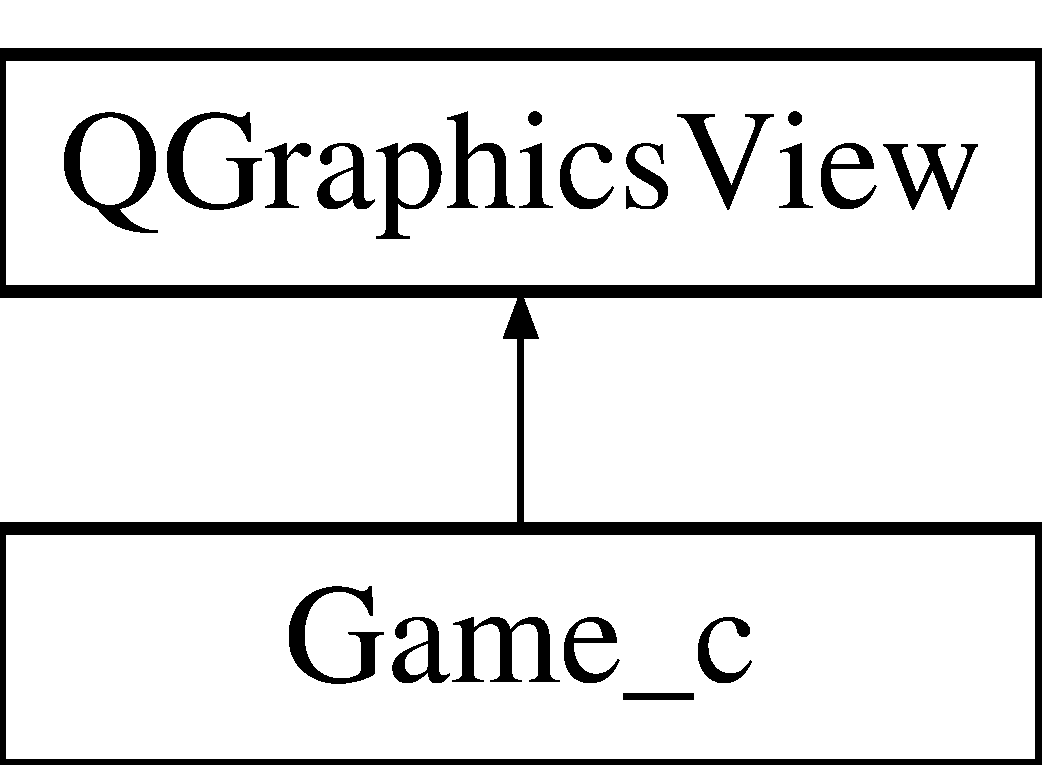
\includegraphics[height=2.000000cm]{classGame__c}
\end{center}
\end{figure}
\subsection*{Slots públicos}
\begin{DoxyCompactItemize}
\item 
\hypertarget{classGame__c_a6a23071ddbebafadca771990d358459b}{void \hyperlink{classGame__c_a6a23071ddbebafadca771990d358459b}{display\-Main\-Menu} ()}\label{classGame__c_a6a23071ddbebafadca771990d358459b}

\begin{DoxyCompactList}\small\item\em Limpia la escena actual y muestra la escena del menú principal. \end{DoxyCompactList}\item 
\hypertarget{classGame__c_a986d16f14b85fc936ae409277386b43d}{void \hyperlink{classGame__c_a986d16f14b85fc936ae409277386b43d}{difficulty\-Selection} ()}\label{classGame__c_a986d16f14b85fc936ae409277386b43d}

\begin{DoxyCompactList}\small\item\em Limpia la escena actual y muestra la escena de selección de dificultad. \end{DoxyCompactList}\item 
\hypertarget{classGame__c_ada099e6da914d235646104b2d6cc0e51}{void \hyperlink{classGame__c_ada099e6da914d235646104b2d6cc0e51}{start} ()}\label{classGame__c_ada099e6da914d235646104b2d6cc0e51}

\begin{DoxyCompactList}\small\item\em Limpia la esena actual e inicia el juego. \end{DoxyCompactList}\item 
\hypertarget{classGame__c_a111258ab784c8a7d75a04e5876a72546}{void \hyperlink{classGame__c_a111258ab784c8a7d75a04e5876a72546}{compare\-\_\-cards} ()}\label{classGame__c_a111258ab784c8a7d75a04e5876a72546}

\begin{DoxyCompactList}\small\item\em Compara las cartas seleccionadas (hacia arriba). \end{DoxyCompactList}\item 
\hypertarget{classGame__c_a02fab778c8803477b80bcc2521778b59}{void \hyperlink{classGame__c_a02fab778c8803477b80bcc2521778b59}{close\-\_\-game} ()}\label{classGame__c_a02fab778c8803477b80bcc2521778b59}

\begin{DoxyCompactList}\small\item\em Cierra el juego y libera la memoria utilizada. \end{DoxyCompactList}\item 
\hypertarget{classGame__c_a99323cea61a4bdde0df2b488f4aff176}{void \hyperlink{classGame__c_a99323cea61a4bdde0df2b488f4aff176}{easy} ()}\label{classGame__c_a99323cea61a4bdde0df2b488f4aff176}

\begin{DoxyCompactList}\small\item\em Modifica el número de pares de cartas a 3. \end{DoxyCompactList}\item 
\hypertarget{classGame__c_af3b1d7d1377731e29a2480795be29ffc}{void \hyperlink{classGame__c_af3b1d7d1377731e29a2480795be29ffc}{medium} ()}\label{classGame__c_af3b1d7d1377731e29a2480795be29ffc}

\begin{DoxyCompactList}\small\item\em Modifica el número de pares de cartas a 5. \end{DoxyCompactList}\item 
\hypertarget{classGame__c_aa75657f3cad93d6fd5516490b7050eba}{void \hyperlink{classGame__c_aa75657f3cad93d6fd5516490b7050eba}{hard} ()}\label{classGame__c_aa75657f3cad93d6fd5516490b7050eba}

\begin{DoxyCompactList}\small\item\em Modifica el número de pares de cartas a 7. \end{DoxyCompactList}\end{DoxyCompactItemize}
\subsection*{Métodos públicos}
\begin{DoxyCompactItemize}
\item 
\hyperlink{classGame__c_a8d6870df89ef4538c92e03a9343770c8}{Game\-\_\-c} (Q\-Graphics\-View $\ast$parent=N\-U\-L\-L)
\begin{DoxyCompactList}\small\item\em Constructor de la clase. \end{DoxyCompactList}\item 
\hypertarget{classGame__c_a67f5de98582607c4c60bca57400bc63a}{void \hyperlink{classGame__c_a67f5de98582607c4c60bca57400bc63a}{display\-Restart\-Game} ()}\label{classGame__c_a67f5de98582607c4c60bca57400bc63a}

\begin{DoxyCompactList}\small\item\em Limpia la escena actual y muestra la escena de juego ganado. \end{DoxyCompactList}\end{DoxyCompactItemize}


\subsection{Descripción detallada}
Clase \hyperlink{classGame__c}{Game\-\_\-c}. Hereda de Q\-Graphics\-View. 

Definición en la línea 40 del archivo game\-\_\-c.\-h.



\subsection{Documentación del constructor y destructor}
\hypertarget{classGame__c_a8d6870df89ef4538c92e03a9343770c8}{\index{Game\-\_\-c@{Game\-\_\-c}!Game\-\_\-c@{Game\-\_\-c}}
\index{Game\-\_\-c@{Game\-\_\-c}!Game_c@{Game\-\_\-c}}
\subsubsection[{Game\-\_\-c}]{\setlength{\rightskip}{0pt plus 5cm}Game\-\_\-c\-::\-Game\-\_\-c (
\begin{DoxyParamCaption}
\item[{Q\-Graphics\-View $\ast$}]{parent = {\ttfamily NULL}}
\end{DoxyParamCaption}
)}}\label{classGame__c_a8d6870df89ef4538c92e03a9343770c8}


Constructor de la clase. 


\begin{DoxyParams}{Parámetros}
{\em parent} & Puntero al Q\-Graphics\-View desde donde se creó esta instancia (N\-U\-L\-L por defecto). \\
\hline
\end{DoxyParams}


Definición en la línea 8 del archivo game\-\_\-c.\-cpp.



La documentación para esta clase fue generada a partir de los siguientes ficheros\-:\begin{DoxyCompactItemize}
\item 
headers/\hyperlink{game__c_8h}{game\-\_\-c.\-h}\item 
source/\hyperlink{game__c_8cpp}{game\-\_\-c.\-cpp}\end{DoxyCompactItemize}

\hypertarget{classGame__r}{\section{Referencia de la Clase Game\-\_\-r}
\label{classGame__r}\index{Game\-\_\-r@{Game\-\_\-r}}
}


Clase \hyperlink{classGame__r}{Game\-\_\-r}. Hereda de Q\-Graphics\-View.  




{\ttfamily \#include $<$game\-\_\-r.\-h$>$}

Diagrama de herencias de Game\-\_\-r\begin{figure}[H]
\begin{center}
\leavevmode
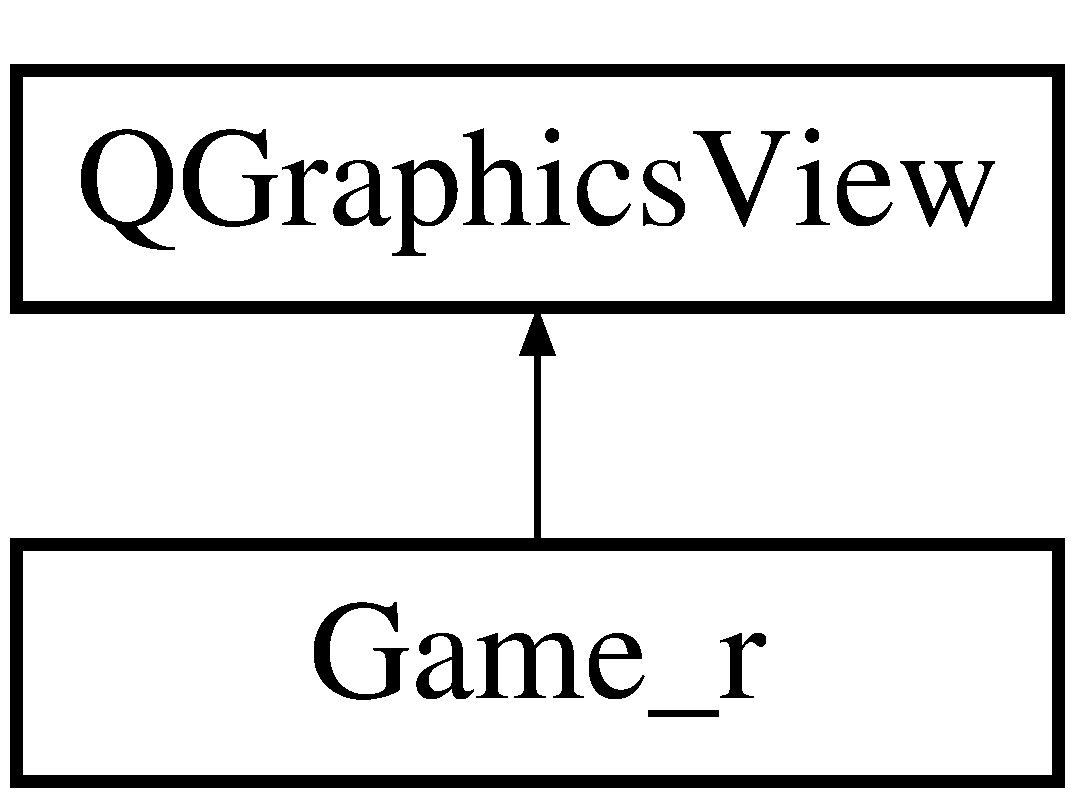
\includegraphics[height=2.000000cm]{classGame__r}
\end{center}
\end{figure}
\subsection*{Slots públicos}
\begin{DoxyCompactItemize}
\item 
\hypertarget{classGame__r_afa9d1405438a52347f726e9aff58c6e8}{void \hyperlink{classGame__r_afa9d1405438a52347f726e9aff58c6e8}{display\-Main\-Menu} ()}\label{classGame__r_afa9d1405438a52347f726e9aff58c6e8}

\begin{DoxyCompactList}\small\item\em Limpia la escena actual y muestra la escena del menú principal. \end{DoxyCompactList}\item 
\hypertarget{classGame__r_a3b39f16df21e7285347a5ce8af4d76e8}{void \hyperlink{classGame__r_a3b39f16df21e7285347a5ce8af4d76e8}{start} ()}\label{classGame__r_a3b39f16df21e7285347a5ce8af4d76e8}

\begin{DoxyCompactList}\small\item\em Limpia la esena actual e inicia el juego. \end{DoxyCompactList}\item 
\hypertarget{classGame__r_afba7fef076f6f41381cc9df2b4837438}{void \hyperlink{classGame__r_afba7fef076f6f41381cc9df2b4837438}{compare\-\_\-cards} ()}\label{classGame__r_afba7fef076f6f41381cc9df2b4837438}

\begin{DoxyCompactList}\small\item\em Compara las cartas seleccionadas (hacia arriba). \end{DoxyCompactList}\item 
\hypertarget{classGame__r_a198360c9ed87d23ffe9ed1ca5c56e946}{void \hyperlink{classGame__r_a198360c9ed87d23ffe9ed1ca5c56e946}{close\-\_\-game} ()}\label{classGame__r_a198360c9ed87d23ffe9ed1ca5c56e946}

\begin{DoxyCompactList}\small\item\em Cierra el juego y libera la memoria utilizada. \end{DoxyCompactList}\end{DoxyCompactItemize}
\subsection*{Métodos públicos}
\begin{DoxyCompactItemize}
\item 
\hyperlink{classGame__r_a4a2fe2cedfd846534bceb9d7db75fd43}{Game\-\_\-r} (Q\-Graphics\-View $\ast$parent=N\-U\-L\-L)
\begin{DoxyCompactList}\small\item\em Constructor de la clase. \end{DoxyCompactList}\item 
\hypertarget{classGame__r_a2dccc96288e21b229267b6c1ecf171a0}{void \hyperlink{classGame__r_a2dccc96288e21b229267b6c1ecf171a0}{display\-Restart\-Game} ()}\label{classGame__r_a2dccc96288e21b229267b6c1ecf171a0}

\begin{DoxyCompactList}\small\item\em Limpia la escena actual y muestra la escena de juego ganado. \end{DoxyCompactList}\item 
\hypertarget{classGame__r_a92dd3f60c8a116cba8db9228582da3de}{void \hyperlink{classGame__r_a92dd3f60c8a116cba8db9228582da3de}{display\-Game\-Over} ()}\label{classGame__r_a92dd3f60c8a116cba8db9228582da3de}

\begin{DoxyCompactList}\small\item\em Limpia la escena actual y muestra la escena de juego perdido. \end{DoxyCompactList}\end{DoxyCompactItemize}


\subsection{Descripción detallada}
Clase \hyperlink{classGame__r}{Game\-\_\-r}. Hereda de Q\-Graphics\-View. 

Definición en la línea 38 del archivo game\-\_\-r.\-h.



\subsection{Documentación del constructor y destructor}
\hypertarget{classGame__r_a4a2fe2cedfd846534bceb9d7db75fd43}{\index{Game\-\_\-r@{Game\-\_\-r}!Game\-\_\-r@{Game\-\_\-r}}
\index{Game\-\_\-r@{Game\-\_\-r}!Game_r@{Game\-\_\-r}}
\subsubsection[{Game\-\_\-r}]{\setlength{\rightskip}{0pt plus 5cm}Game\-\_\-r\-::\-Game\-\_\-r (
\begin{DoxyParamCaption}
\item[{Q\-Graphics\-View $\ast$}]{parent = {\ttfamily NULL}}
\end{DoxyParamCaption}
)}}\label{classGame__r_a4a2fe2cedfd846534bceb9d7db75fd43}


Constructor de la clase. 


\begin{DoxyParams}{Parámetros}
{\em parent} & Puntero al Q\-Graphics\-View desde donde se creó esta instancia (N\-U\-L\-L por defecto). \\
\hline
\end{DoxyParams}


Definición en la línea 8 del archivo game\-\_\-r.\-cpp.



La documentación para esta clase fue generada a partir de los siguientes ficheros\-:\begin{DoxyCompactItemize}
\item 
headers/\hyperlink{game__r_8h}{game\-\_\-r.\-h}\item 
source/\hyperlink{game__r_8cpp}{game\-\_\-r.\-cpp}\end{DoxyCompactItemize}

\hypertarget{classgame__select}{\section{Referencia de la Clase game\-\_\-select}
\label{classgame__select}\index{game\-\_\-select@{game\-\_\-select}}
}
Diagrama de herencias de game\-\_\-select\begin{figure}[H]
\begin{center}
\leavevmode
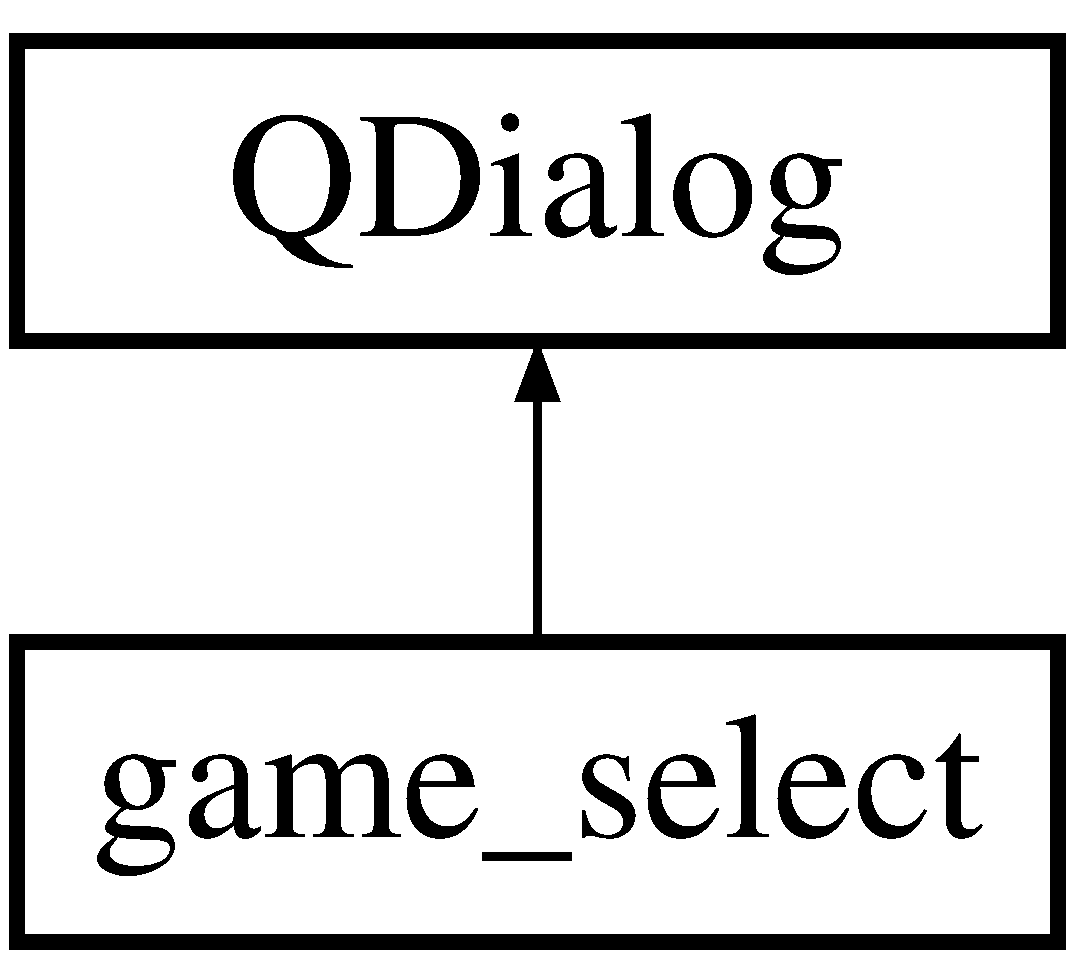
\includegraphics[height=2.000000cm]{classgame__select}
\end{center}
\end{figure}
\subsection*{Métodos públicos}
\begin{DoxyCompactItemize}
\item 
\hypertarget{classgame__select_a2fa0dae60cdc46a56e4ffd941976cd88}{{\bfseries game\-\_\-select} (Q\-Widget $\ast$parent=0)}\label{classgame__select_a2fa0dae60cdc46a56e4ffd941976cd88}

\end{DoxyCompactItemize}


\subsection{Descripción detallada}


Definición en la línea 18 del archivo game\-\_\-select.\-h.



La documentación para esta clase fue generada a partir de los siguientes ficheros\-:\begin{DoxyCompactItemize}
\item 
headers/\hyperlink{game__select_8h}{game\-\_\-select.\-h}\item 
source/\hyperlink{game__select_8cpp}{game\-\_\-select.\-cpp}\end{DoxyCompactItemize}

\hypertarget{classMainWindow}{\section{Referencia de la Clase Main\-Window}
\label{classMainWindow}\index{Main\-Window@{Main\-Window}}
}
Diagrama de herencias de Main\-Window\begin{figure}[H]
\begin{center}
\leavevmode
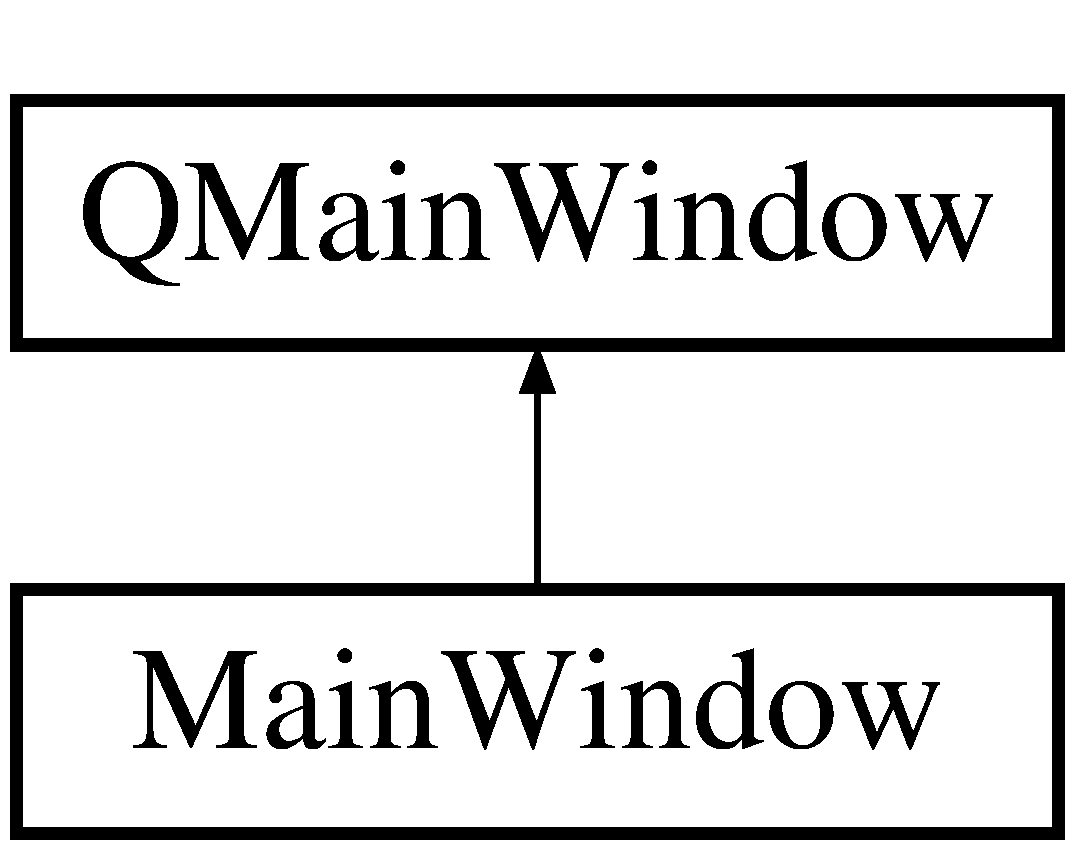
\includegraphics[height=2.000000cm]{classMainWindow}
\end{center}
\end{figure}
\subsection*{Métodos públicos}
\begin{DoxyCompactItemize}
\item 
\hypertarget{classMainWindow_a8b244be8b7b7db1b08de2a2acb9409db}{{\bfseries Main\-Window} (Q\-Widget $\ast$parent=0)}\label{classMainWindow_a8b244be8b7b7db1b08de2a2acb9409db}

\end{DoxyCompactItemize}


\subsection{Descripción detallada}


Definición en la línea 18 del archivo mainwindow.\-h.



La documentación para esta clase fue generada a partir de los siguientes ficheros\-:\begin{DoxyCompactItemize}
\item 
headers/\hyperlink{mainwindow_8h}{mainwindow.\-h}\item 
source/\hyperlink{mainwindow_8cpp}{mainwindow.\-cpp}\end{DoxyCompactItemize}

\chapter{Documentación de archivos}
\hypertarget{about_8h}{\section{Referencia del Archivo headers/about.h}
\label{about_8h}\index{headers/about.\-h@{headers/about.\-h}}
}
{\ttfamily \#include $<$Q\-Dialog$>$}\\*
\subsection*{Clases}
\begin{DoxyCompactItemize}
\item 
class \hyperlink{classabout}{about}
\end{DoxyCompactItemize}


\subsection{Descripción detallada}
\begin{DoxyAuthor}{Autor}
Angel España -\/ Git\-Hub aespaben 

Patricia Daboin -\/ Git\-Hub apdaboin 
\end{DoxyAuthor}


Definición en el archivo \hyperlink{about_8h_source}{about.\-h}.


\hypertarget{aux__functions_8h}{\section{Referencia del Archivo headers/aux\-\_\-functions.h}
\label{aux__functions_8h}\index{headers/aux\-\_\-functions.\-h@{headers/aux\-\_\-functions.\-h}}
}
{\ttfamily \#include $<$Q\-Dir\-Iterator$>$}\\*
{\ttfamily \#include $<$Q\-Pixmap$>$}\\*
{\ttfamily \#include $<$cstdlib$>$}\\*
{\ttfamily \#include $<$time.\-h$>$}\\*
{\ttfamily \#include $<$list.\-H$>$}\\*
{\ttfamily \#include \char`\"{}headers/\-Card.\-h\char`\"{}}\\*
\subsection*{Funciones}
\begin{DoxyCompactItemize}
\item 
void \hyperlink{aux__functions_8h_a87d8be954310ef0279c1aa2a08e59888}{random\-\_\-pos\-\_\-numbers\-\_\-array} (int a\mbox{[}$\,$\mbox{]}, size\-\_\-t a\-\_\-size)
\begin{DoxyCompactList}\small\item\em Recibe un arreglo de números enteros (vacío) y le añade números enteros aleatorios sin repetir entre 0 y a\-\_\-size. \end{DoxyCompactList}\item 
{\footnotesize template$<$typename T $>$ }\\void \hyperlink{aux__functions_8h_ab8c70cca28e16967e860b44baf2bec7f}{random\-\_\-array} (T a\mbox{[}$\,$\mbox{]}, size\-\_\-t a\-\_\-size)
\begin{DoxyCompactList}\small\item\em Aleatoriza las posiciones de los elementos de un arreglo cualquiera. \end{DoxyCompactList}\item 
void \hyperlink{aux__functions_8h_a31456360c93cd842ad2ac01863440993}{random\-\_\-array} (S\-L\-List$<$ Q\-String $>$ $\ast$a, size\-\_\-t a\-\_\-size)
\begin{DoxyCompactList}\small\item\em Aleatoriza las posiciones de los elementos de una lista simplemente enlazada. \end{DoxyCompactList}\item 
void \hyperlink{aux__functions_8h_ab4f3011775fa80aacdffbe381419ced9}{random\-\_\-array} (\hyperlink{classCard}{Card} $\ast$c\mbox{[}$\,$\mbox{]}, size\-\_\-t c\-\_\-size)
\begin{DoxyCompactList}\small\item\em Aleatoriza las posiciones de los elementos de un arreglo de tipo Card$\ast$. \end{DoxyCompactList}\item 
void \hyperlink{aux__functions_8h_a6225eb37d6182d1b698033a0a31bd865}{load\-\_\-random\-\_\-pixmaps\-\_\-from\-\_\-dir} (Q\-Pixmap p\mbox{[}$\,$\mbox{]}, size\-\_\-t p\-\_\-size, Q\-String qs\-\_\-dir)
\begin{DoxyCompactList}\small\item\em Carga imágenes aleatorias a un arreglo de tipo Q\-Pixmap de acuerdo a una ubicación específica. \end{DoxyCompactList}\item 
void \hyperlink{aux__functions_8h_ad8829af29a0805d9270d95f43385f676}{load\-\_\-random\-\_\-pixmaps\-\_\-from\-\_\-dir} (S\-L\-List$<$ Q\-String $>$ $\ast$sll\-\_\-files, size\-\_\-t p\-\_\-size, Q\-String qs\-\_\-dir)
\begin{DoxyCompactList}\small\item\em Carga path's de imágenes aleatorias a una lista simplemente enlazada de tipo Q\-Pixmap de acuerdo a una ubicación específica. \end{DoxyCompactList}\end{DoxyCompactItemize}


\subsection{Descripción detallada}
\begin{DoxyAuthor}{Autor}
Angel España -\/ Git\-Hub aespaben 

Patricia Daboin -\/ Git\-Hub apdaboin 
\end{DoxyAuthor}


Definición en el archivo \hyperlink{aux__functions_8h_source}{aux\-\_\-functions.\-h}.



\subsection{Documentación de las funciones}
\hypertarget{aux__functions_8h_a6225eb37d6182d1b698033a0a31bd865}{\index{aux\-\_\-functions.\-h@{aux\-\_\-functions.\-h}!load\-\_\-random\-\_\-pixmaps\-\_\-from\-\_\-dir@{load\-\_\-random\-\_\-pixmaps\-\_\-from\-\_\-dir}}
\index{load\-\_\-random\-\_\-pixmaps\-\_\-from\-\_\-dir@{load\-\_\-random\-\_\-pixmaps\-\_\-from\-\_\-dir}!aux_functions.h@{aux\-\_\-functions.\-h}}
\subsubsection[{load\-\_\-random\-\_\-pixmaps\-\_\-from\-\_\-dir}]{\setlength{\rightskip}{0pt plus 5cm}void load\-\_\-random\-\_\-pixmaps\-\_\-from\-\_\-dir (
\begin{DoxyParamCaption}
\item[{Q\-Pixmap}]{p\mbox{[}$\,$\mbox{]}, }
\item[{size\-\_\-t}]{p\-\_\-size, }
\item[{Q\-String}]{qs\-\_\-dir}
\end{DoxyParamCaption}
)}}\label{aux__functions_8h_a6225eb37d6182d1b698033a0a31bd865}


Carga imágenes aleatorias a un arreglo de tipo Q\-Pixmap de acuerdo a una ubicación específica. 


\begin{DoxyParams}{Parámetros}
{\em p} & Arreglo de imágenes (vacío). \\
\hline
{\em p\-\_\-size} & Tamaño del arreglo. \\
\hline
{\em qs\-\_\-dir} & Path del directorio donde se ubican las imágenes. \\
\hline
\end{DoxyParams}


Definición en la línea 128 del archivo aux\-\_\-functions.\-cpp.

\hypertarget{aux__functions_8h_ad8829af29a0805d9270d95f43385f676}{\index{aux\-\_\-functions.\-h@{aux\-\_\-functions.\-h}!load\-\_\-random\-\_\-pixmaps\-\_\-from\-\_\-dir@{load\-\_\-random\-\_\-pixmaps\-\_\-from\-\_\-dir}}
\index{load\-\_\-random\-\_\-pixmaps\-\_\-from\-\_\-dir@{load\-\_\-random\-\_\-pixmaps\-\_\-from\-\_\-dir}!aux_functions.h@{aux\-\_\-functions.\-h}}
\subsubsection[{load\-\_\-random\-\_\-pixmaps\-\_\-from\-\_\-dir}]{\setlength{\rightskip}{0pt plus 5cm}void load\-\_\-random\-\_\-pixmaps\-\_\-from\-\_\-dir (
\begin{DoxyParamCaption}
\item[{S\-L\-List$<$ Q\-String $>$ $\ast$}]{sll\-\_\-files, }
\item[{size\-\_\-t}]{p\-\_\-size, }
\item[{Q\-String}]{qs\-\_\-dir}
\end{DoxyParamCaption}
)}}\label{aux__functions_8h_ad8829af29a0805d9270d95f43385f676}


Carga path's de imágenes aleatorias a una lista simplemente enlazada de tipo Q\-Pixmap de acuerdo a una ubicación específica. 


\begin{DoxyParams}{Parámetros}
{\em sll\-\_\-files} & Lista simplemente enlazada (puede estar vacía o no). \\
\hline
{\em p\-\_\-size} & Cantidad de imágenes a cargar. \\
\hline
{\em qs\-\_\-dir} & Path del directorio donde se ubican las imágenes. \\
\hline
\end{DoxyParams}


Definición en la línea 143 del archivo aux\-\_\-functions.\-cpp.

\hypertarget{aux__functions_8h_ab8c70cca28e16967e860b44baf2bec7f}{\index{aux\-\_\-functions.\-h@{aux\-\_\-functions.\-h}!random\-\_\-array@{random\-\_\-array}}
\index{random\-\_\-array@{random\-\_\-array}!aux_functions.h@{aux\-\_\-functions.\-h}}
\subsubsection[{random\-\_\-array}]{\setlength{\rightskip}{0pt plus 5cm}template$<$typename T $>$ void random\-\_\-array (
\begin{DoxyParamCaption}
\item[{T}]{a\mbox{[}$\,$\mbox{]}, }
\item[{size\-\_\-t}]{a\-\_\-size}
\end{DoxyParamCaption}
)}}\label{aux__functions_8h_ab8c70cca28e16967e860b44baf2bec7f}


Aleatoriza las posiciones de los elementos de un arreglo cualquiera. 


\begin{DoxyParams}{Parámetros}
{\em a} & Arreglo de cualquier tipo. \\
\hline
{\em a\-\_\-size} & Tamaño del arreglo a\mbox{[}\mbox{]}. \\
\hline
\end{DoxyParams}


Definición en la línea 33 del archivo aux\-\_\-functions.\-cpp.

\hypertarget{aux__functions_8h_a31456360c93cd842ad2ac01863440993}{\index{aux\-\_\-functions.\-h@{aux\-\_\-functions.\-h}!random\-\_\-array@{random\-\_\-array}}
\index{random\-\_\-array@{random\-\_\-array}!aux_functions.h@{aux\-\_\-functions.\-h}}
\subsubsection[{random\-\_\-array}]{\setlength{\rightskip}{0pt plus 5cm}void random\-\_\-array (
\begin{DoxyParamCaption}
\item[{S\-L\-List$<$ Q\-String $>$ $\ast$}]{a, }
\item[{size\-\_\-t}]{a\-\_\-size}
\end{DoxyParamCaption}
)}}\label{aux__functions_8h_a31456360c93cd842ad2ac01863440993}


Aleatoriza las posiciones de los elementos de una lista simplemente enlazada. 


\begin{DoxyParams}{Parámetros}
{\em a} & Lista simplemente enlazada. \\
\hline
{\em a\-\_\-size} & Tamaño de la lista a. \\
\hline
\end{DoxyParams}


Definición en la línea 65 del archivo aux\-\_\-functions.\-cpp.

\hypertarget{aux__functions_8h_ab4f3011775fa80aacdffbe381419ced9}{\index{aux\-\_\-functions.\-h@{aux\-\_\-functions.\-h}!random\-\_\-array@{random\-\_\-array}}
\index{random\-\_\-array@{random\-\_\-array}!aux_functions.h@{aux\-\_\-functions.\-h}}
\subsubsection[{random\-\_\-array}]{\setlength{\rightskip}{0pt plus 5cm}void random\-\_\-array (
\begin{DoxyParamCaption}
\item[{{\bf Card} $\ast$}]{c\mbox{[}$\,$\mbox{]}, }
\item[{size\-\_\-t}]{c\-\_\-size}
\end{DoxyParamCaption}
)}}\label{aux__functions_8h_ab4f3011775fa80aacdffbe381419ced9}


Aleatoriza las posiciones de los elementos de un arreglo de tipo Card$\ast$. 


\begin{DoxyParams}{Parámetros}
{\em c} & Arreglo de tipo Card$\ast$. \\
\hline
{\em c\-\_\-size} & Tamaño del arreglo c. \\
\hline
\end{DoxyParams}


Definición en la línea 96 del archivo aux\-\_\-functions.\-cpp.

\hypertarget{aux__functions_8h_a87d8be954310ef0279c1aa2a08e59888}{\index{aux\-\_\-functions.\-h@{aux\-\_\-functions.\-h}!random\-\_\-pos\-\_\-numbers\-\_\-array@{random\-\_\-pos\-\_\-numbers\-\_\-array}}
\index{random\-\_\-pos\-\_\-numbers\-\_\-array@{random\-\_\-pos\-\_\-numbers\-\_\-array}!aux_functions.h@{aux\-\_\-functions.\-h}}
\subsubsection[{random\-\_\-pos\-\_\-numbers\-\_\-array}]{\setlength{\rightskip}{0pt plus 5cm}void random\-\_\-pos\-\_\-numbers\-\_\-array (
\begin{DoxyParamCaption}
\item[{int}]{a\mbox{[}$\,$\mbox{]}, }
\item[{size\-\_\-t}]{a\-\_\-size}
\end{DoxyParamCaption}
)}}\label{aux__functions_8h_a87d8be954310ef0279c1aa2a08e59888}


Recibe un arreglo de números enteros (vacío) y le añade números enteros aleatorios sin repetir entre 0 y a\-\_\-size. 


\begin{DoxyParams}{Parámetros}
{\em a} & Arreglo de números enteros \\
\hline
{\em a\-\_\-size} & Tamaño del arreglo a\mbox{[}\mbox{]}. \\
\hline
\end{DoxyParams}


Definición en la línea 8 del archivo aux\-\_\-functions.\-cpp.


\hypertarget{button_8h}{\section{Referencia del Archivo headers/button.h}
\label{button_8h}\index{headers/button.\-h@{headers/button.\-h}}
}
{\ttfamily \#include $<$Q\-Graphics\-Rect\-Item$>$}\\*
{\ttfamily \#include $<$Q\-Graphics\-Scene\-Mouse\-Event$>$}\\*
{\ttfamily \#include $<$Q\-Brush$>$}\\*
\subsection*{Clases}
\begin{DoxyCompactItemize}
\item 
class \hyperlink{classButton}{Button}
\begin{DoxyCompactList}\small\item\em Clase \hyperlink{classButton}{Button}. Hereda de Q\-Object y Q\-Graphics\-Pixmap\-Item. \end{DoxyCompactList}\end{DoxyCompactItemize}


\subsection{Descripción detallada}
\begin{DoxyAuthor}{Autor}
Angel España -\/ Git\-Hub aespaben 

Patricia Daboin -\/ Git\-Hub apdaboin 
\end{DoxyAuthor}


Definición en el archivo \hyperlink{button_8h_source}{button.\-h}.


\hypertarget{Card_8h}{\section{Referencia del Archivo headers/\-Card.h}
\label{Card_8h}\index{headers/\-Card.\-h@{headers/\-Card.\-h}}
}
{\ttfamily \#include $<$Q\-Pixmap$>$}\\*
{\ttfamily \#include $<$Q\-Graphics\-Pixmap\-Item$>$}\\*
{\ttfamily \#include $<$Q\-Graphics\-Scene\-Mouse\-Event$>$}\\*
\subsection*{Clases}
\begin{DoxyCompactItemize}
\item 
class \hyperlink{classCard}{Card}
\begin{DoxyCompactList}\small\item\em Clase \hyperlink{classCard}{Card}. Hereda de Q\-Object y Q\-Graphics\-Pixmap\-Item. \end{DoxyCompactList}\end{DoxyCompactItemize}


\subsection{Descripción detallada}
\begin{DoxyAuthor}{Autor}
Angel España -\/ Git\-Hub aespaben 

Patricia Daboin -\/ Git\-Hub apdaboin 
\end{DoxyAuthor}


Definición en el archivo \hyperlink{Card_8h_source}{Card.\-h}.


\hypertarget{game__c_8h}{\section{Referencia del Archivo headers/game\-\_\-c.h}
\label{game__c_8h}\index{headers/game\-\_\-c.\-h@{headers/game\-\_\-c.\-h}}
}
{\ttfamily \#include $<$Q\-Desktop\-Widget$>$}\\*
{\ttfamily \#include $<$Q\-Application$>$}\\*
{\ttfamily \#include $<$Q\-Graphics\-Scene$>$}\\*
{\ttfamily \#include $<$Q\-Graphics\-View$>$}\\*
{\ttfamily \#include $<$Q\-Timer$>$}\\*
{\ttfamily \#include $<$Q\-Thread$>$}\\*
{\ttfamily \#include $<$Q\-List$>$}\\*
{\ttfamily \#include $<$Q\-Icon$>$}\\*
{\ttfamily \#include $<$Q\-Dialog$>$}\\*
{\ttfamily \#include $<$graph.\-H$>$}\\*
{\ttfamily \#include $<$list.\-H$>$}\\*
{\ttfamily \#include $<$cstdlib$>$}\\*
{\ttfamily \#include $<$time.\-h$>$}\\*
{\ttfamily \#include $<$headers/aux\-\_\-functions.\-h$>$}\\*
{\ttfamily \#include $<$headers/\-Card.\-h$>$}\\*
{\ttfamily \#include $<$headers/button.\-h$>$}\\*
{\ttfamily \#include $<$headers/game\-\_\-select.\-h$>$}\\*
\subsection*{Clases}
\begin{DoxyCompactItemize}
\item 
class \hyperlink{classGame__c}{Game\-\_\-c}
\begin{DoxyCompactList}\small\item\em Clase \hyperlink{classGame__c}{Game\-\_\-c}. Hereda de Q\-Graphics\-View. \end{DoxyCompactList}\end{DoxyCompactItemize}
\subsection*{'defines'}
\begin{DoxyCompactItemize}
\item 
\hypertarget{game__c_8h_afd2537d19a3cb6556b0f727580ec6ee7}{\#define {\bfseries S\-I\-Z\-E}(x)~(sizeof(x)/sizeof(x\mbox{[}0\mbox{]}))}\label{game__c_8h_afd2537d19a3cb6556b0f727580ec6ee7}

\end{DoxyCompactItemize}
\subsection*{'typedefs'}
\begin{DoxyCompactItemize}
\item 
\hypertarget{game__c_8h_a1b5e76b9d080414c5e989c824ff6f2fa}{using {\bfseries Deck} = Graph$<$ \hyperlink{classCard}{Card} $\ast$, int $>$}\label{game__c_8h_a1b5e76b9d080414c5e989c824ff6f2fa}

\end{DoxyCompactItemize}


\subsection{Descripción detallada}
\begin{DoxyAuthor}{Autor}
Angel España -\/ Git\-Hub aespaben 

Patricia Daboin -\/ Git\-Hub apdaboin 
\end{DoxyAuthor}


Definición en el archivo \hyperlink{game__c_8h_source}{game\-\_\-c.\-h}.


\hypertarget{game__r_8h}{\section{Referencia del Archivo headers/game\-\_\-r.h}
\label{game__r_8h}\index{headers/game\-\_\-r.\-h@{headers/game\-\_\-r.\-h}}
}
{\ttfamily \#include $<$Q\-Desktop\-Widget$>$}\\*
{\ttfamily \#include $<$Q\-Application$>$}\\*
{\ttfamily \#include $<$Q\-Graphics\-Scene$>$}\\*
{\ttfamily \#include $<$Q\-Graphics\-View$>$}\\*
{\ttfamily \#include $<$Q\-Thread$>$}\\*
{\ttfamily \#include $<$Q\-List$>$}\\*
{\ttfamily \#include $<$Q\-Icon$>$}\\*
{\ttfamily \#include $<$graph.\-H$>$}\\*
{\ttfamily \#include $<$list.\-H$>$}\\*
{\ttfamily \#include $<$cstdlib$>$}\\*
{\ttfamily \#include $<$time.\-h$>$}\\*
{\ttfamily \#include $<$headers/aux\-\_\-functions.\-h$>$}\\*
{\ttfamily \#include $<$headers/\-Card.\-h$>$}\\*
{\ttfamily \#include $<$headers/button.\-h$>$}\\*
{\ttfamily \#include $<$headers/game\-\_\-select.\-h$>$}\\*
\subsection*{Clases}
\begin{DoxyCompactItemize}
\item 
class \hyperlink{classGame__r}{Game\-\_\-r}
\begin{DoxyCompactList}\small\item\em Clase \hyperlink{classGame__r}{Game\-\_\-r}. Hereda de Q\-Graphics\-View. \end{DoxyCompactList}\end{DoxyCompactItemize}
\subsection*{'defines'}
\begin{DoxyCompactItemize}
\item 
\hypertarget{game__r_8h_afd2537d19a3cb6556b0f727580ec6ee7}{\#define {\bfseries S\-I\-Z\-E}(x)~(sizeof(x)/sizeof(x\mbox{[}0\mbox{]}))}\label{game__r_8h_afd2537d19a3cb6556b0f727580ec6ee7}

\end{DoxyCompactItemize}
\subsection*{'typedefs'}
\begin{DoxyCompactItemize}
\item 
\hypertarget{game__r_8h_a1b5e76b9d080414c5e989c824ff6f2fa}{using {\bfseries Deck} = Graph$<$ \hyperlink{classCard}{Card} $\ast$, int $>$}\label{game__r_8h_a1b5e76b9d080414c5e989c824ff6f2fa}

\end{DoxyCompactItemize}


\subsection{Descripción detallada}
\begin{DoxyAuthor}{Autor}
Angel España -\/ Git\-Hub aespaben 

Patricia Daboin -\/ Git\-Hub apdaboin 
\end{DoxyAuthor}


Definición en el archivo \hyperlink{game__r_8h_source}{game\-\_\-r.\-h}.


\hypertarget{game__select_8h}{\section{Referencia del Archivo headers/game\-\_\-select.h}
\label{game__select_8h}\index{headers/game\-\_\-select.\-h@{headers/game\-\_\-select.\-h}}
}
{\ttfamily \#include $<$Q\-Dialog$>$}\\*
{\ttfamily \#include \char`\"{}headers/mainwindow.\-h\char`\"{}}\\*
{\ttfamily \#include \char`\"{}headers/game\-\_\-c.\-h\char`\"{}}\\*
{\ttfamily \#include \char`\"{}headers/game\-\_\-r.\-h\char`\"{}}\\*
\subsection*{Clases}
\begin{DoxyCompactItemize}
\item 
class \hyperlink{classgame__select}{game\-\_\-select}
\end{DoxyCompactItemize}


\subsection{Descripción detallada}
\begin{DoxyAuthor}{Autor}
Angel España -\/ Git\-Hub aespaben 

Patricia Daboin -\/ Git\-Hub apdaboin 
\end{DoxyAuthor}


Definición en el archivo \hyperlink{game__select_8h_source}{game\-\_\-select.\-h}.


\hypertarget{mainwindow_8h}{\section{Referencia del Archivo headers/mainwindow.h}
\label{mainwindow_8h}\index{headers/mainwindow.\-h@{headers/mainwindow.\-h}}
}
{\ttfamily \#include $<$Q\-Main\-Window$>$}\\*
{\ttfamily \#include $<$Q\-Desktop\-Widget$>$}\\*
{\ttfamily \#include $<$headers/game\-\_\-select.\-h$>$}\\*
{\ttfamily \#include $<$headers/about.\-h$>$}\\*
\subsection*{Clases}
\begin{DoxyCompactItemize}
\item 
class \hyperlink{classMainWindow}{Main\-Window}
\end{DoxyCompactItemize}


\subsection{Descripción detallada}
\begin{DoxyAuthor}{Autor}
Angel España -\/ Git\-Hub aespaben 

Patricia Daboin -\/ Git\-Hub apdaboin 
\end{DoxyAuthor}


Definición en el archivo \hyperlink{mainwindow_8h_source}{mainwindow.\-h}.


\hypertarget{about_8cpp}{\section{Referencia del Archivo source/about.cpp}
\label{about_8cpp}\index{source/about.\-cpp@{source/about.\-cpp}}
}
{\ttfamily \#include \char`\"{}headers/about.\-h\char`\"{}}\\*
{\ttfamily \#include \char`\"{}ui\-\_\-about.\-h\char`\"{}}\\*


\subsection{Descripción detallada}
\begin{DoxyAuthor}{Autor}
Angel España -\/ Git\-Hub aespaben 

Patricia Daboin -\/ Git\-Hub apdaboin 
\end{DoxyAuthor}


Definición en el archivo \hyperlink{about_8cpp_source}{about.\-cpp}.


\hypertarget{aux__functions_8cpp}{\section{Referencia del Archivo source/aux\-\_\-functions.cpp}
\label{aux__functions_8cpp}\index{source/aux\-\_\-functions.\-cpp@{source/aux\-\_\-functions.\-cpp}}
}
{\ttfamily \#include $<$headers/aux\-\_\-functions.\-h$>$}\\*
\subsection*{Funciones}
\begin{DoxyCompactItemize}
\item 
void \hyperlink{aux__functions_8cpp_a87d8be954310ef0279c1aa2a08e59888}{random\-\_\-pos\-\_\-numbers\-\_\-array} (int a\mbox{[}$\,$\mbox{]}, size\-\_\-t a\-\_\-size)
\begin{DoxyCompactList}\small\item\em Recibe un arreglo de números enteros (vacío) y le añade números enteros aleatorios sin repetir entre 0 y a\-\_\-size. \end{DoxyCompactList}\item 
{\footnotesize template$<$typename T $>$ }\\void \hyperlink{aux__functions_8cpp_ab8c70cca28e16967e860b44baf2bec7f}{random\-\_\-array} (T a\mbox{[}$\,$\mbox{]}, size\-\_\-t a\-\_\-size)
\begin{DoxyCompactList}\small\item\em Aleatoriza las posiciones de los elementos de un arreglo cualquiera. \end{DoxyCompactList}\item 
void \hyperlink{aux__functions_8cpp_a31456360c93cd842ad2ac01863440993}{random\-\_\-array} (S\-L\-List$<$ Q\-String $>$ $\ast$a, size\-\_\-t a\-\_\-size)
\begin{DoxyCompactList}\small\item\em Aleatoriza las posiciones de los elementos de una lista simplemente enlazada. \end{DoxyCompactList}\item 
void \hyperlink{aux__functions_8cpp_ab4f3011775fa80aacdffbe381419ced9}{random\-\_\-array} (\hyperlink{classCard}{Card} $\ast$c\mbox{[}$\,$\mbox{]}, size\-\_\-t c\-\_\-size)
\begin{DoxyCompactList}\small\item\em Aleatoriza las posiciones de los elementos de un arreglo de tipo Card$\ast$. \end{DoxyCompactList}\item 
void \hyperlink{aux__functions_8cpp_a6225eb37d6182d1b698033a0a31bd865}{load\-\_\-random\-\_\-pixmaps\-\_\-from\-\_\-dir} (Q\-Pixmap p\mbox{[}$\,$\mbox{]}, size\-\_\-t p\-\_\-size, Q\-String qs\-\_\-dir)
\begin{DoxyCompactList}\small\item\em Carga imágenes aleatorias a un arreglo de tipo Q\-Pixmap de acuerdo a una ubicación específica. \end{DoxyCompactList}\item 
void \hyperlink{aux__functions_8cpp_aa3b13667f4c928508a1ec52495c6e9e0}{load\-\_\-random\-\_\-pixmaps\-\_\-from\-\_\-dir} (S\-L\-List$<$ Q\-String $>$ $\ast$sll\-\_\-files, size\-\_\-t l\-\_\-size, Q\-String qs\-\_\-dir)
\begin{DoxyCompactList}\small\item\em Carga path's de imágenes aleatorias a una lista simplemente enlazada de tipo Q\-Pixmap de acuerdo a una ubicación específica. \end{DoxyCompactList}\end{DoxyCompactItemize}


\subsection{Descripción detallada}
\begin{DoxyAuthor}{Autor}
Angel España -\/ Git\-Hub aespaben 

Patricia Daboin -\/ Git\-Hub apdaboin 
\end{DoxyAuthor}


Definición en el archivo \hyperlink{aux__functions_8cpp_source}{aux\-\_\-functions.\-cpp}.



\subsection{Documentación de las funciones}
\hypertarget{aux__functions_8cpp_a6225eb37d6182d1b698033a0a31bd865}{\index{aux\-\_\-functions.\-cpp@{aux\-\_\-functions.\-cpp}!load\-\_\-random\-\_\-pixmaps\-\_\-from\-\_\-dir@{load\-\_\-random\-\_\-pixmaps\-\_\-from\-\_\-dir}}
\index{load\-\_\-random\-\_\-pixmaps\-\_\-from\-\_\-dir@{load\-\_\-random\-\_\-pixmaps\-\_\-from\-\_\-dir}!aux_functions.cpp@{aux\-\_\-functions.\-cpp}}
\subsubsection[{load\-\_\-random\-\_\-pixmaps\-\_\-from\-\_\-dir}]{\setlength{\rightskip}{0pt plus 5cm}void load\-\_\-random\-\_\-pixmaps\-\_\-from\-\_\-dir (
\begin{DoxyParamCaption}
\item[{Q\-Pixmap}]{p\mbox{[}$\,$\mbox{]}, }
\item[{size\-\_\-t}]{p\-\_\-size, }
\item[{Q\-String}]{qs\-\_\-dir}
\end{DoxyParamCaption}
)}}\label{aux__functions_8cpp_a6225eb37d6182d1b698033a0a31bd865}


Carga imágenes aleatorias a un arreglo de tipo Q\-Pixmap de acuerdo a una ubicación específica. 


\begin{DoxyParams}{Parámetros}
{\em p} & Arreglo de imágenes (vacío). \\
\hline
{\em p\-\_\-size} & Tamaño del arreglo. \\
\hline
{\em qs\-\_\-dir} & Path del directorio donde se ubican las imágenes. \\
\hline
\end{DoxyParams}


Definición en la línea 128 del archivo aux\-\_\-functions.\-cpp.

\hypertarget{aux__functions_8cpp_aa3b13667f4c928508a1ec52495c6e9e0}{\index{aux\-\_\-functions.\-cpp@{aux\-\_\-functions.\-cpp}!load\-\_\-random\-\_\-pixmaps\-\_\-from\-\_\-dir@{load\-\_\-random\-\_\-pixmaps\-\_\-from\-\_\-dir}}
\index{load\-\_\-random\-\_\-pixmaps\-\_\-from\-\_\-dir@{load\-\_\-random\-\_\-pixmaps\-\_\-from\-\_\-dir}!aux_functions.cpp@{aux\-\_\-functions.\-cpp}}
\subsubsection[{load\-\_\-random\-\_\-pixmaps\-\_\-from\-\_\-dir}]{\setlength{\rightskip}{0pt plus 5cm}void load\-\_\-random\-\_\-pixmaps\-\_\-from\-\_\-dir (
\begin{DoxyParamCaption}
\item[{S\-L\-List$<$ Q\-String $>$ $\ast$}]{sll\-\_\-files, }
\item[{size\-\_\-t}]{p\-\_\-size, }
\item[{Q\-String}]{qs\-\_\-dir}
\end{DoxyParamCaption}
)}}\label{aux__functions_8cpp_aa3b13667f4c928508a1ec52495c6e9e0}


Carga path's de imágenes aleatorias a una lista simplemente enlazada de tipo Q\-Pixmap de acuerdo a una ubicación específica. 


\begin{DoxyParams}{Parámetros}
{\em sll\-\_\-files} & Lista simplemente enlazada (puede estar vacía o no). \\
\hline
{\em p\-\_\-size} & Cantidad de imágenes a cargar. \\
\hline
{\em qs\-\_\-dir} & Path del directorio donde se ubican las imágenes. \\
\hline
\end{DoxyParams}


Definición en la línea 143 del archivo aux\-\_\-functions.\-cpp.

\hypertarget{aux__functions_8cpp_ab8c70cca28e16967e860b44baf2bec7f}{\index{aux\-\_\-functions.\-cpp@{aux\-\_\-functions.\-cpp}!random\-\_\-array@{random\-\_\-array}}
\index{random\-\_\-array@{random\-\_\-array}!aux_functions.cpp@{aux\-\_\-functions.\-cpp}}
\subsubsection[{random\-\_\-array}]{\setlength{\rightskip}{0pt plus 5cm}template$<$typename T $>$ void random\-\_\-array (
\begin{DoxyParamCaption}
\item[{T}]{a\mbox{[}$\,$\mbox{]}, }
\item[{size\-\_\-t}]{a\-\_\-size}
\end{DoxyParamCaption}
)}}\label{aux__functions_8cpp_ab8c70cca28e16967e860b44baf2bec7f}


Aleatoriza las posiciones de los elementos de un arreglo cualquiera. 


\begin{DoxyParams}{Parámetros}
{\em a} & Arreglo de cualquier tipo. \\
\hline
{\em a\-\_\-size} & Tamaño del arreglo a\mbox{[}\mbox{]}. \\
\hline
\end{DoxyParams}


Definición en la línea 33 del archivo aux\-\_\-functions.\-cpp.

\hypertarget{aux__functions_8cpp_a31456360c93cd842ad2ac01863440993}{\index{aux\-\_\-functions.\-cpp@{aux\-\_\-functions.\-cpp}!random\-\_\-array@{random\-\_\-array}}
\index{random\-\_\-array@{random\-\_\-array}!aux_functions.cpp@{aux\-\_\-functions.\-cpp}}
\subsubsection[{random\-\_\-array}]{\setlength{\rightskip}{0pt plus 5cm}void random\-\_\-array (
\begin{DoxyParamCaption}
\item[{S\-L\-List$<$ Q\-String $>$ $\ast$}]{a, }
\item[{size\-\_\-t}]{a\-\_\-size}
\end{DoxyParamCaption}
)}}\label{aux__functions_8cpp_a31456360c93cd842ad2ac01863440993}


Aleatoriza las posiciones de los elementos de una lista simplemente enlazada. 


\begin{DoxyParams}{Parámetros}
{\em a} & Lista simplemente enlazada. \\
\hline
{\em a\-\_\-size} & Tamaño de la lista a. \\
\hline
\end{DoxyParams}


Definición en la línea 65 del archivo aux\-\_\-functions.\-cpp.

\hypertarget{aux__functions_8cpp_ab4f3011775fa80aacdffbe381419ced9}{\index{aux\-\_\-functions.\-cpp@{aux\-\_\-functions.\-cpp}!random\-\_\-array@{random\-\_\-array}}
\index{random\-\_\-array@{random\-\_\-array}!aux_functions.cpp@{aux\-\_\-functions.\-cpp}}
\subsubsection[{random\-\_\-array}]{\setlength{\rightskip}{0pt plus 5cm}void random\-\_\-array (
\begin{DoxyParamCaption}
\item[{{\bf Card} $\ast$}]{c\mbox{[}$\,$\mbox{]}, }
\item[{size\-\_\-t}]{c\-\_\-size}
\end{DoxyParamCaption}
)}}\label{aux__functions_8cpp_ab4f3011775fa80aacdffbe381419ced9}


Aleatoriza las posiciones de los elementos de un arreglo de tipo Card$\ast$. 


\begin{DoxyParams}{Parámetros}
{\em c} & Arreglo de tipo Card$\ast$. \\
\hline
{\em c\-\_\-size} & Tamaño del arreglo c. \\
\hline
\end{DoxyParams}


Definición en la línea 96 del archivo aux\-\_\-functions.\-cpp.

\hypertarget{aux__functions_8cpp_a87d8be954310ef0279c1aa2a08e59888}{\index{aux\-\_\-functions.\-cpp@{aux\-\_\-functions.\-cpp}!random\-\_\-pos\-\_\-numbers\-\_\-array@{random\-\_\-pos\-\_\-numbers\-\_\-array}}
\index{random\-\_\-pos\-\_\-numbers\-\_\-array@{random\-\_\-pos\-\_\-numbers\-\_\-array}!aux_functions.cpp@{aux\-\_\-functions.\-cpp}}
\subsubsection[{random\-\_\-pos\-\_\-numbers\-\_\-array}]{\setlength{\rightskip}{0pt plus 5cm}void random\-\_\-pos\-\_\-numbers\-\_\-array (
\begin{DoxyParamCaption}
\item[{int}]{a\mbox{[}$\,$\mbox{]}, }
\item[{size\-\_\-t}]{a\-\_\-size}
\end{DoxyParamCaption}
)}}\label{aux__functions_8cpp_a87d8be954310ef0279c1aa2a08e59888}


Recibe un arreglo de números enteros (vacío) y le añade números enteros aleatorios sin repetir entre 0 y a\-\_\-size. 


\begin{DoxyParams}{Parámetros}
{\em a} & Arreglo de números enteros \\
\hline
{\em a\-\_\-size} & Tamaño del arreglo a\mbox{[}\mbox{]}. \\
\hline
\end{DoxyParams}


Definición en la línea 8 del archivo aux\-\_\-functions.\-cpp.


\hypertarget{button_8cpp}{\section{Referencia del Archivo source/button.cpp}
\label{button_8cpp}\index{source/button.\-cpp@{source/button.\-cpp}}
}
{\ttfamily \#include \char`\"{}headers/button.\-h\char`\"{}}\\*


\subsection{Descripción detallada}
\begin{DoxyAuthor}{Autor}
Angel España -\/ Git\-Hub aespaben 

Patricia Daboin -\/ Git\-Hub apdaboin 
\end{DoxyAuthor}


Definición en el archivo \hyperlink{button_8cpp_source}{button.\-cpp}.


\hypertarget{game__c_8cpp}{\section{Referencia del Archivo source/game\-\_\-c.cpp}
\label{game__c_8cpp}\index{source/game\-\_\-c.\-cpp@{source/game\-\_\-c.\-cpp}}
}
{\ttfamily \#include \char`\"{}headers/game\-\_\-c.\-h\char`\"{}}\\*


\subsection{Descripción detallada}
\begin{DoxyAuthor}{Autor}
Angel España -\/ Git\-Hub aespaben 

Patricia Daboin -\/ Git\-Hub apdaboin 
\end{DoxyAuthor}


Definición en el archivo \hyperlink{game__c_8cpp_source}{game\-\_\-c.\-cpp}.


\hypertarget{game__r_8cpp}{\section{Referencia del Archivo source/game\-\_\-r.cpp}
\label{game__r_8cpp}\index{source/game\-\_\-r.\-cpp@{source/game\-\_\-r.\-cpp}}
}
{\ttfamily \#include \char`\"{}headers/game\-\_\-r.\-h\char`\"{}}\\*


\subsection{Descripción detallada}
\begin{DoxyAuthor}{Autor}
Angel España -\/ Git\-Hub aespaben 

Patricia Daboin -\/ Git\-Hub apdaboin 
\end{DoxyAuthor}


Definición en el archivo \hyperlink{game__r_8cpp_source}{game\-\_\-r.\-cpp}.


\hypertarget{game__select_8cpp}{\section{Referencia del Archivo source/game\-\_\-select.cpp}
\label{game__select_8cpp}\index{source/game\-\_\-select.\-cpp@{source/game\-\_\-select.\-cpp}}
}
{\ttfamily \#include \char`\"{}headers/game\-\_\-select.\-h\char`\"{}}\\*
{\ttfamily \#include \char`\"{}ui\-\_\-game\-\_\-select.\-h\char`\"{}}\\*


\subsection{Descripción detallada}
\begin{DoxyAuthor}{Autor}
Angel España -\/ Git\-Hub aespaben 

Patricia Daboin -\/ Git\-Hub apdaboin 
\end{DoxyAuthor}


Definición en el archivo \hyperlink{game__select_8cpp_source}{game\-\_\-select.\-cpp}.


\hypertarget{main_8cpp}{\section{Referencia del Archivo source/main.cpp}
\label{main_8cpp}\index{source/main.\-cpp@{source/main.\-cpp}}
}
{\ttfamily \#include \char`\"{}headers/mainwindow.\-h\char`\"{}}\\*
{\ttfamily \#include $<$Q\-Application$>$}\\*
\subsection*{Funciones}
\begin{DoxyCompactItemize}
\item 
\hypertarget{main_8cpp_a0ddf1224851353fc92bfbff6f499fa97}{int {\bfseries main} (int argc, char $\ast$argv\mbox{[}$\,$\mbox{]})}\label{main_8cpp_a0ddf1224851353fc92bfbff6f499fa97}

\end{DoxyCompactItemize}


\subsection{Descripción detallada}
\begin{DoxyAuthor}{Autor}
Angel España -\/ Git\-Hub aespaben 

Patricia Daboin -\/ Git\-Hub apdaboin 
\end{DoxyAuthor}


Definición en el archivo \hyperlink{main_8cpp_source}{main.\-cpp}.


\hypertarget{mainwindow_8cpp}{\section{Referencia del Archivo source/mainwindow.cpp}
\label{mainwindow_8cpp}\index{source/mainwindow.\-cpp@{source/mainwindow.\-cpp}}
}
{\ttfamily \#include \char`\"{}headers/mainwindow.\-h\char`\"{}}\\*
{\ttfamily \#include \char`\"{}ui\-\_\-mainwindow.\-h\char`\"{}}\\*


\subsection{Descripción detallada}
\begin{DoxyAuthor}{Autor}
Angel España -\/ Git\-Hub aespaben 

Patricia Daboin -\/ Git\-Hub apdaboin 
\end{DoxyAuthor}


Definición en el archivo \hyperlink{mainwindow_8cpp_source}{mainwindow.\-cpp}.


%--- End generated contents ---

% Index
\newpage
\phantomsection
\addcontentsline{toc}{chapter}{Índice}
\printindex

\end{document}
